\chapter{Applications of TDA}
\graphicspath{ {/home/tomasp/Dokumenty/Master_Thesis/figures/} }

In this section, we will go over some of the more popular methods, techniques and algorithms that are used within Topological Data Analysis. The most theoretically demanding one is Persistent Homology that we worked on introducing in the previous chapters in the most basic and stripped down manner to not overwhelm the reader. We will look at the popular clustering and dimensionality reducing algorithms such as UMAP and Mapper, both closely related to each other. In the direction of homology, we will look at other equivalent and potentially more useful representations such as persistence images, landscapes and entropy. We will demonstrate them on the classical setting of point clouds but also time series and graphs.

All methods will be accompanied by examples, both toy examples to better understand and real-life data to show one can use the methods to obtain new information. It is hopelessly naive to believe that we can summarize all the ways TDA and its surrounding methods have been and can be used to. As such, the reader will be pointed to different articles that cover more intricate applications that go beyond the scope of this work.

\section{UMAP}
UMAP, short for \textit{Uniform Manifold Approximation and Projection for Dimension Reduction}, is a dimension reduction technique, similar to something like t-SNE, that is commonly used for dataset visualization, clustering, filtering or embedding within neural networks. UMAP and Mapper complement each other and are usually used together, hence why we talk about UMAP first.

UMAP is built on three, relatively reasonable, assumptions about your dataset:
\begin{itemize}
  \item The data is uniformly distributed on a Riemannian manifold.
  \item The Riemannian metric is locally constant or can be approximated as such.
  \item The Riemannian manifold is locally connected.
\end{itemize}

If the assumptions are satisfied, it is then possible to model the ambient manifold with what we call a \textit{fuzzy} topological structure. We will briefly explain and summarize the workings of the algorithm, although it is recommended to read the original article \cite{mcinnes2020umapuniformmanifoldapproximation} for a more detailed explanation.

The first step is to approximate the manifold the data supposedly lies on. Assuming that the manifold isn't known in advance (perhaps from some theoretical description of the model), we need to approximate the geodesic distance. It simplifies the problem to assume that the data is uniformly distributed on the manifold. Given this, we can center balls of an appropriate radius around each point to obtain a crude approximation of the manifold. We can then approximate geodesic distances from each ball to its neighbour.

Unfortunately, this means that we have independent notions of distances that may or may not be compatible. To merge all the local metric spaces into one compatible global structure, we utilize fuzzy simplicial sets, where a fuzzy set is characterized by a carrier set $A$ and a map $\mu: A \to [0,1]$ we call the membership function. This turns membership from a property attaining two values -- true or false -- into a property taking values in the unit interval. Each metric space is translated into a fuzzy simplicial set via a categorical construction (the fuzzy singular set functor).

The goal, once we have constructed our fuzzy simplicial set, is to find a low-dimensional representation of our data that closely matches the topological structure. This optimal embedding is found after minimizing the error between the two representations with respect to cross entropy of the fuzzy sets. From a purely computational perspective, UMAP can be described in terms of weighted graphs; placing UMAP in the class of graph learning algorithms such as Isomap, the above-mentioned t-SNE and Laplacian Eigenmaps.

We will go over some examples of UMAP on well-known datasets and later compare the obtained results with the one we will see with Mapper in the next section.

\subsection{Penguin dataset}
We will start with a simple example using the known Penguin dataset \cite{10.1371/journal.pone.0090081}. The simplicity of the dataset will make it easier to highlight and interpret the results from UMAP. The dataset has few features, as seen in \ref{tab:penguins}, with some data missing and replaced with NaNs. While it would be recommended to use some form of imputation to replace them in a proper study, we will simply drop the missing values in this example without worrying too much.

The dataset itself contains measurements about bill dimensions and flipper lengths, alongside metadata regarding the penguin's body mass and sex. The values we will focus on are the first four, ignoring the species and island variables. There are a total of 333 penguins in this dataset, and we can start with a simple pairwise scatter plot matrix to get a rough idea of what we're dealing with, seen in \ref{fig:penguins_scatter}

\begin{table}[]
\centering
\resizebox{\textwidth}{!}{%
\begin{tabular}{|c|c|c|c|c|c|c|c|c|}
\hline
 &
  \textbf{species} &
  \textbf{island} &
  \textbf{bill\_length\_mm} &
  \textbf{bill\_depth\_mm} &
  \textbf{flipper\_length\_mm} &
  \textbf{body\_mass\_g} &
  \textbf{sex} &
  \textbf{year} \\ \hline
0 & Adelie & Torgersen & 39.1 & 18.7 & 181.0 & 3750.0 & male   & 2007 \\ \hline
1 & Adelie & Torgersen & 39.5 & 17.4 & 186.0 & 3800.0 & female & 2007 \\ \hline
2 & Adelie & Torgersen & 40.3 & 18.0 & 195.0 & 3250.0 & female & 2007 \\ \hline
3 & Adelie & Torgersen & NaN  & NaN  & NaN   & NaN    & NaN    & 2007 \\ \hline
4 & Adelie & Torgersen & 36.7 & 19.3 & 193.0 & 3450.0 & female & 2007 \\ \hline
\end{tabular}%
}
\caption{First five rows of the Penguin dataset.}
\label{tab:penguins}
\end{table}

\begin{figure}[h!]
  \centering
  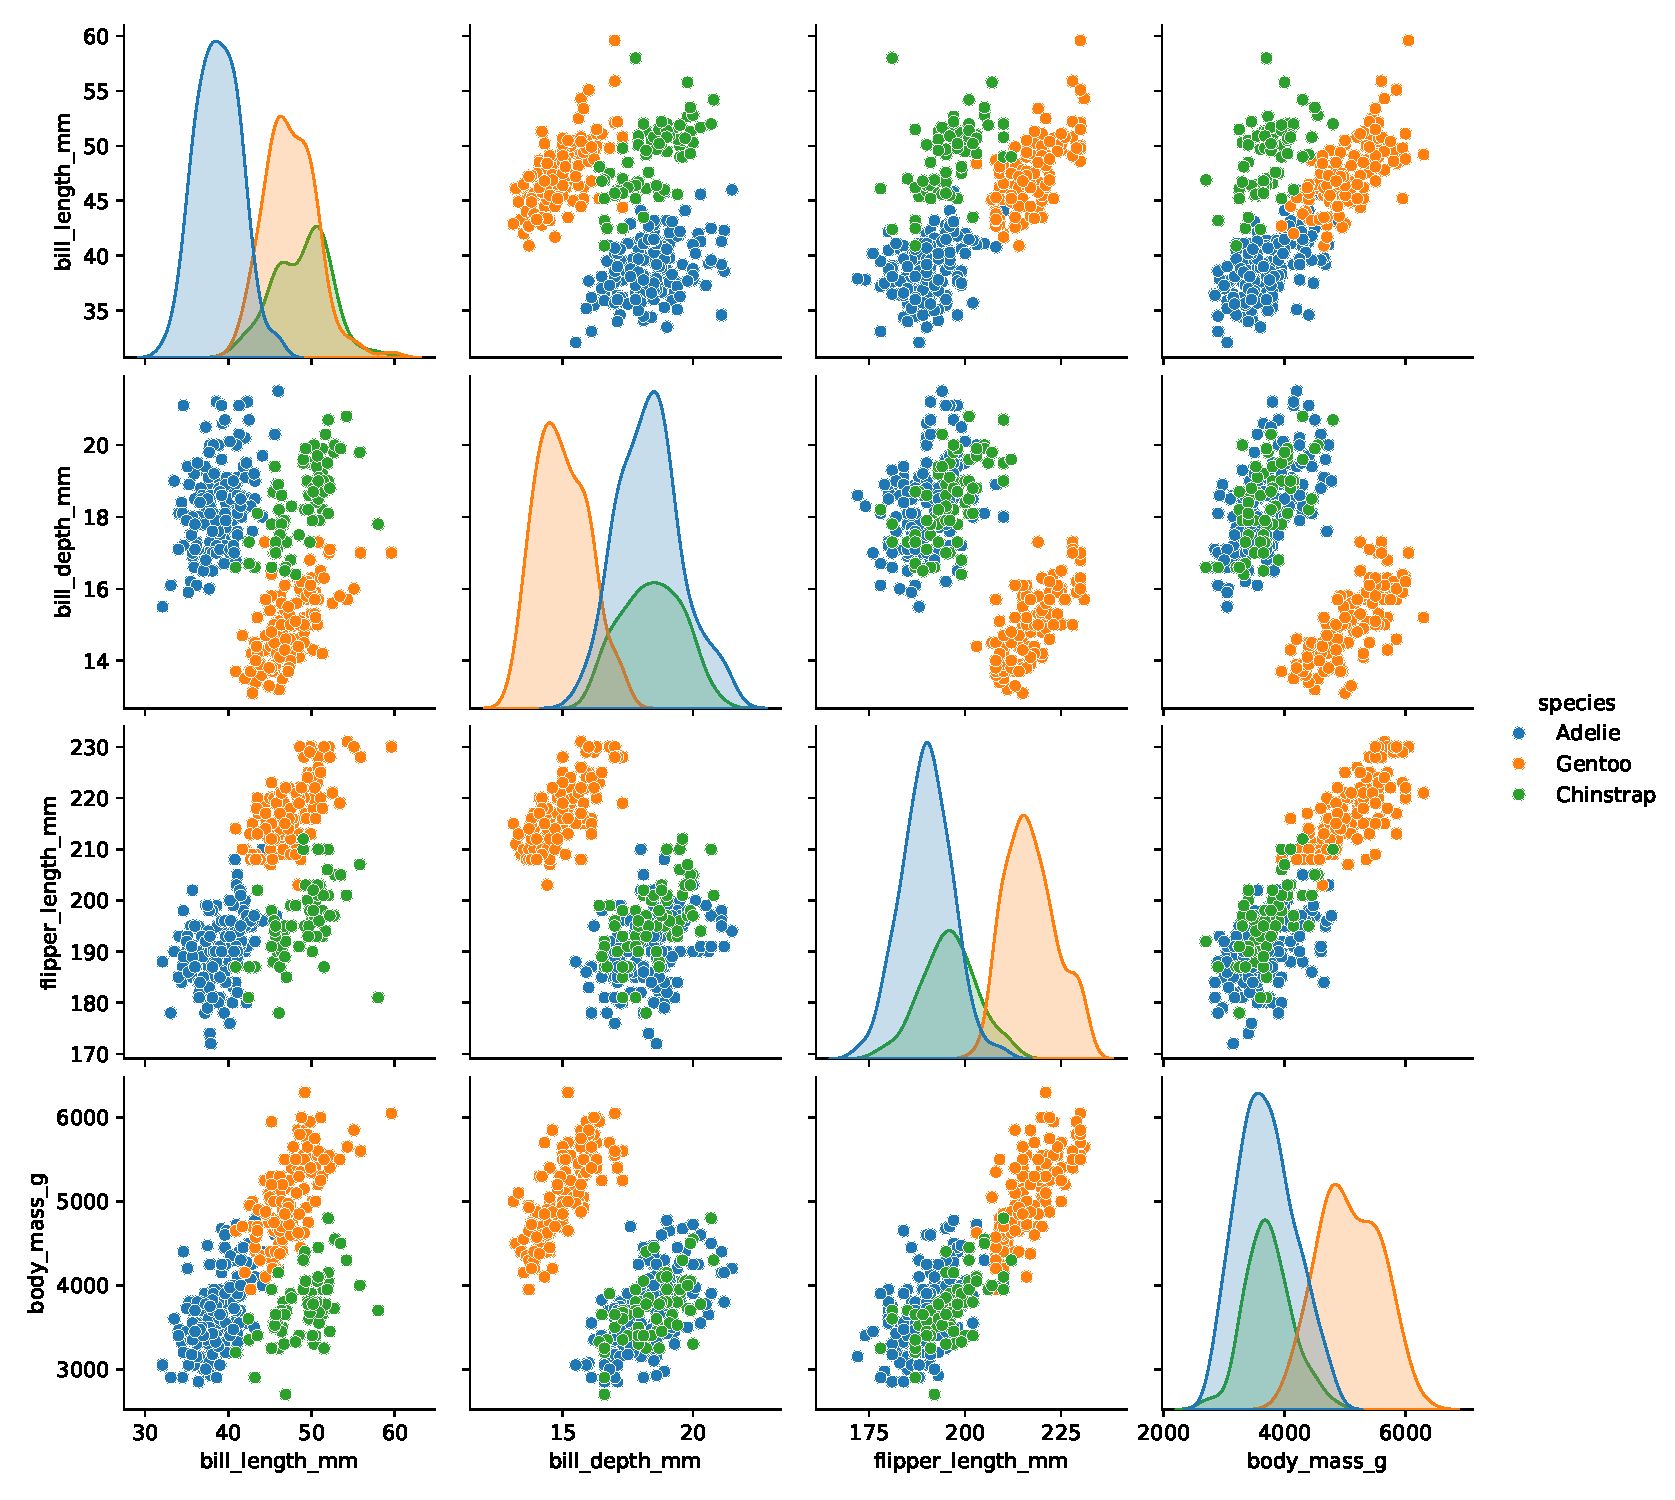
\includegraphics[width=15cm, height=13.5cm]{Penguins_scatterplot.pdf}
  \caption{Pairwise plots of the Penguin dataset for the bill length, bill depth, flipper length and body mass variables.}
  \label{fig:penguins_scatter}
\end{figure}

For this task, we will use the Python library UMAP \cite{mcinnes2018umap-software} to reduce the dimension in a way that preserves the topology of the 4-dimensional space we are working with. We can first remove the missing values and the columns we won't need for this short analysis. Since we are working with different scales, it is generally useful to convert the features into z-scores or use a different scaler process.

\begin{figure}[h!]
  \centering
  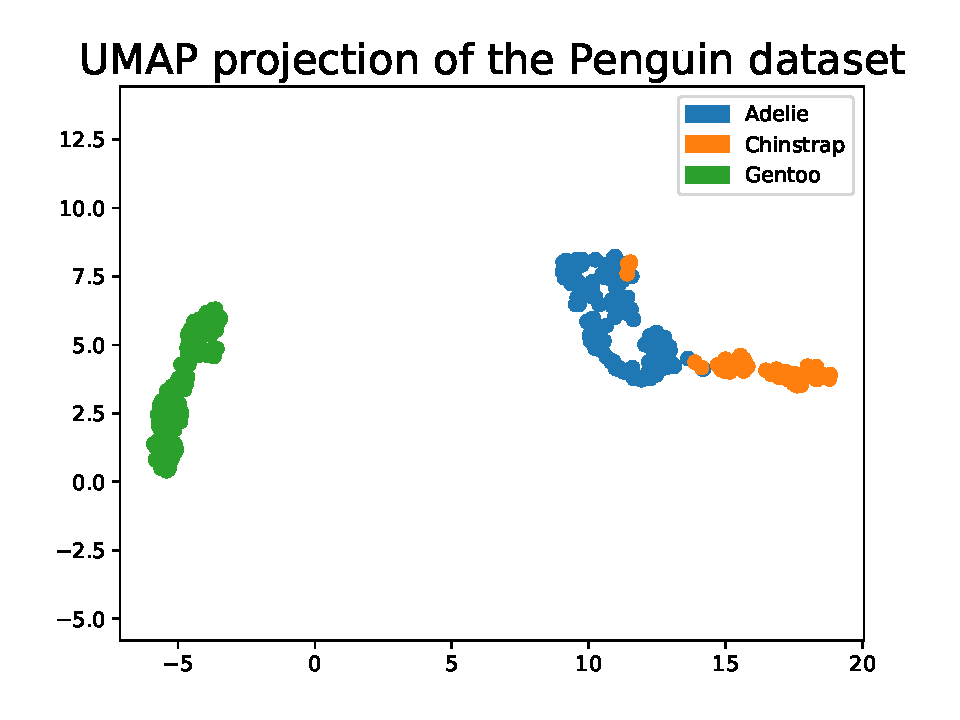
\includegraphics[width=12cm, height=10cm]{penguins_projection.pdf}
  \caption{UMAP dimension reduction result on the Penguin dataset.}
  \label{fig:penguins_projection}
\end{figure}

The result of reducing the dimension can be seen in \ref{fig:penguins_projection}. Comparing it to \ref{fig:penguins_scatter}, it does a good job of capturing the relationships between the three groups. Although, in this case specifically, we already found everything we needed in the scatter plot matrix, which was only possible because we worked with four dimensions. Once the number of features is higher, a scatter plot matrix becomes unwieldy and difficult to read properly.

\subsection{Digits dataset}
For an example with a high number of features, we can consider the known digits dataset \cite{optical_recognition_of_handwritten_digits_80}, one of the many toy datasets used to validate both old and new algorithms. We can iterate over the individual images to display them on a grid in \ref{fig:digits} to see what we are working with.

\begin{figure}[h!]
  \centering
  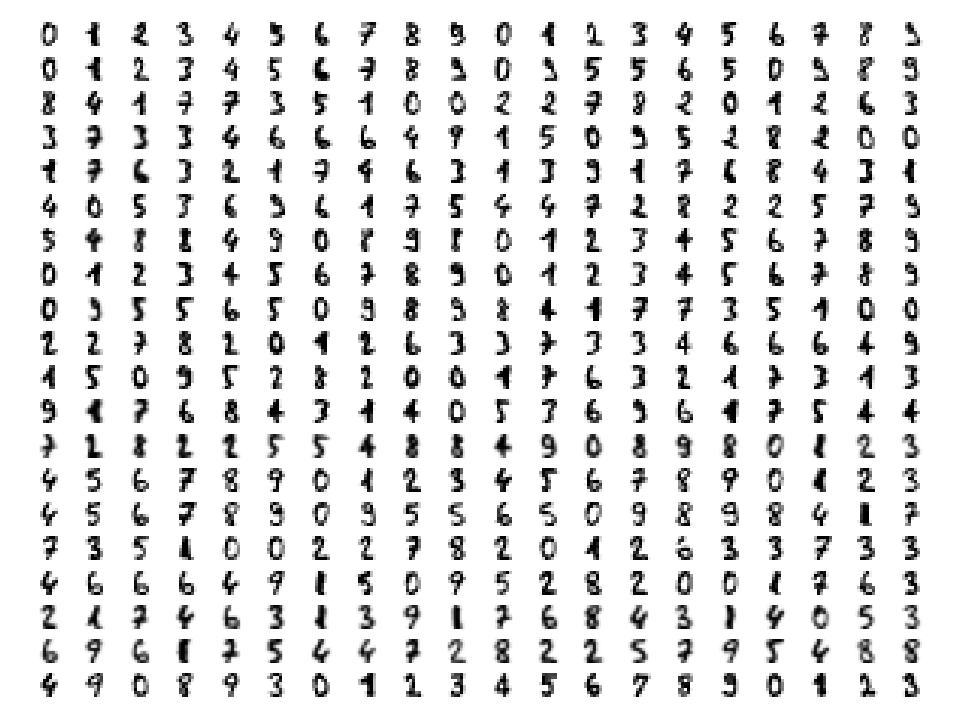
\includegraphics[width=12cm, height=10cm]{digits.pdf}
  \caption{First few images of the digits dataset}
  \label{fig:digits}
\end{figure}

The digits dataset contains 1797 bitmaps of hand-written digits in 10 classes -- each class corresponding to its digit. Most digits are somewhat readable but there are few that are simply too blurred to be considered useful for any further analysis. Such bitmaps should be separated into their own cluster of outliers, creating one additional class in the end.
The usual goal is to classify and cluster each bitmap into its appropriate class. We will see that with UMAP, we obtain satisfying results with a simple application of the algorithm. We see in \ref{fig:digits_projection} that reducing the dimension with UMAP already gave us a rather solid clustering of the digits with significant clusters. It shouldn't come off as a suprise that fairly distinct digits like 0, 9, 2, 6 or 7 are far away from the rest; whereas digits 1, 8, 3 lie close to each other.

\begin{figure}[h!]
  \centering
  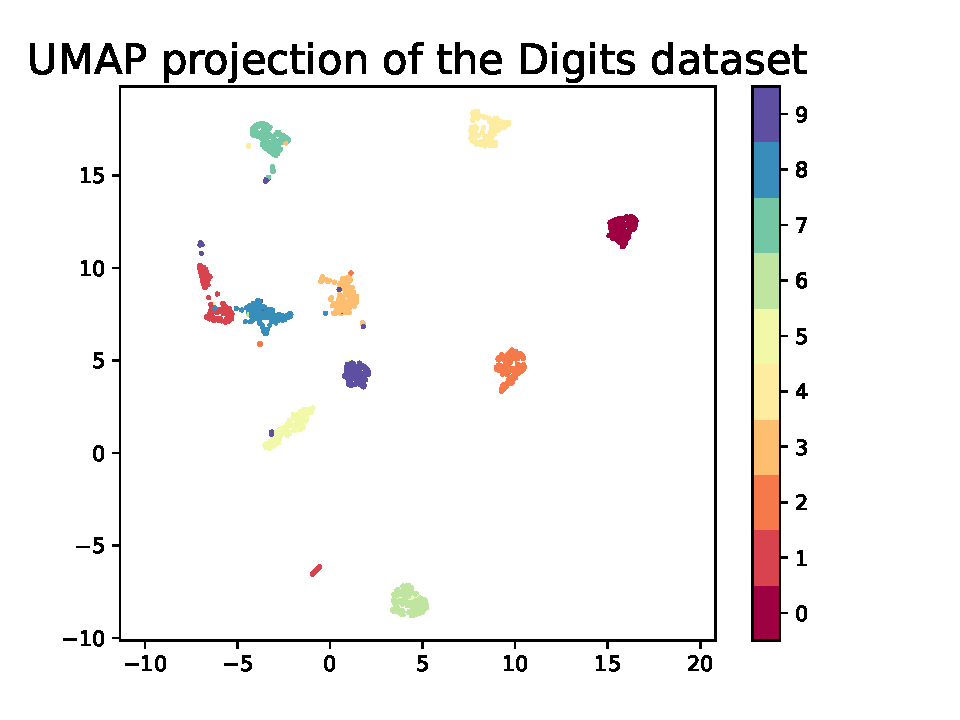
\includegraphics[width=12cm, height=11cm]{digits_projection.pdf}
  \caption{Result of UMAP on the digits dataset.}
  \label{fig:digits_projection}
\end{figure}

We will look into the digits dataset two more times -- once with Mapper in the next section and the second time using homology groups instead.

\subsection{Fashion and clothes}
We can look at a much larger dataset to see how UMAP compares. Fashion-MNIST \cite{DBLP:journals/corr/abs-1708-07747} is a dataset consisting of 60,000 examples of Zelando's clothing articles, each article being a 28x28 grayscale image associated to one of 10 classes. The classes go as follow, labelled from 0 to 9 -- T-shirt, Trouser, Pullover, Dress, Coat, Sandal, Shirt, Sneaker, Bag, and Ankle Boot.
As was the case for the digits dataset, one is typically interested in classifying and clustering the clothing articles while removing the images that are too blurred. Applying UMAP, we can see the resulting projection on \ref{fig:fmnist}. On a more technical note, the MNIST dataset should be ideally replaced with a different one since it is too easy for modern machine learning algorithms, is usually overused and cannot represent modern Computer Vision tasks. But since this text isn't about Computer Vision, we can safely proceed.

\begin{figure}[h!]
  \centering
  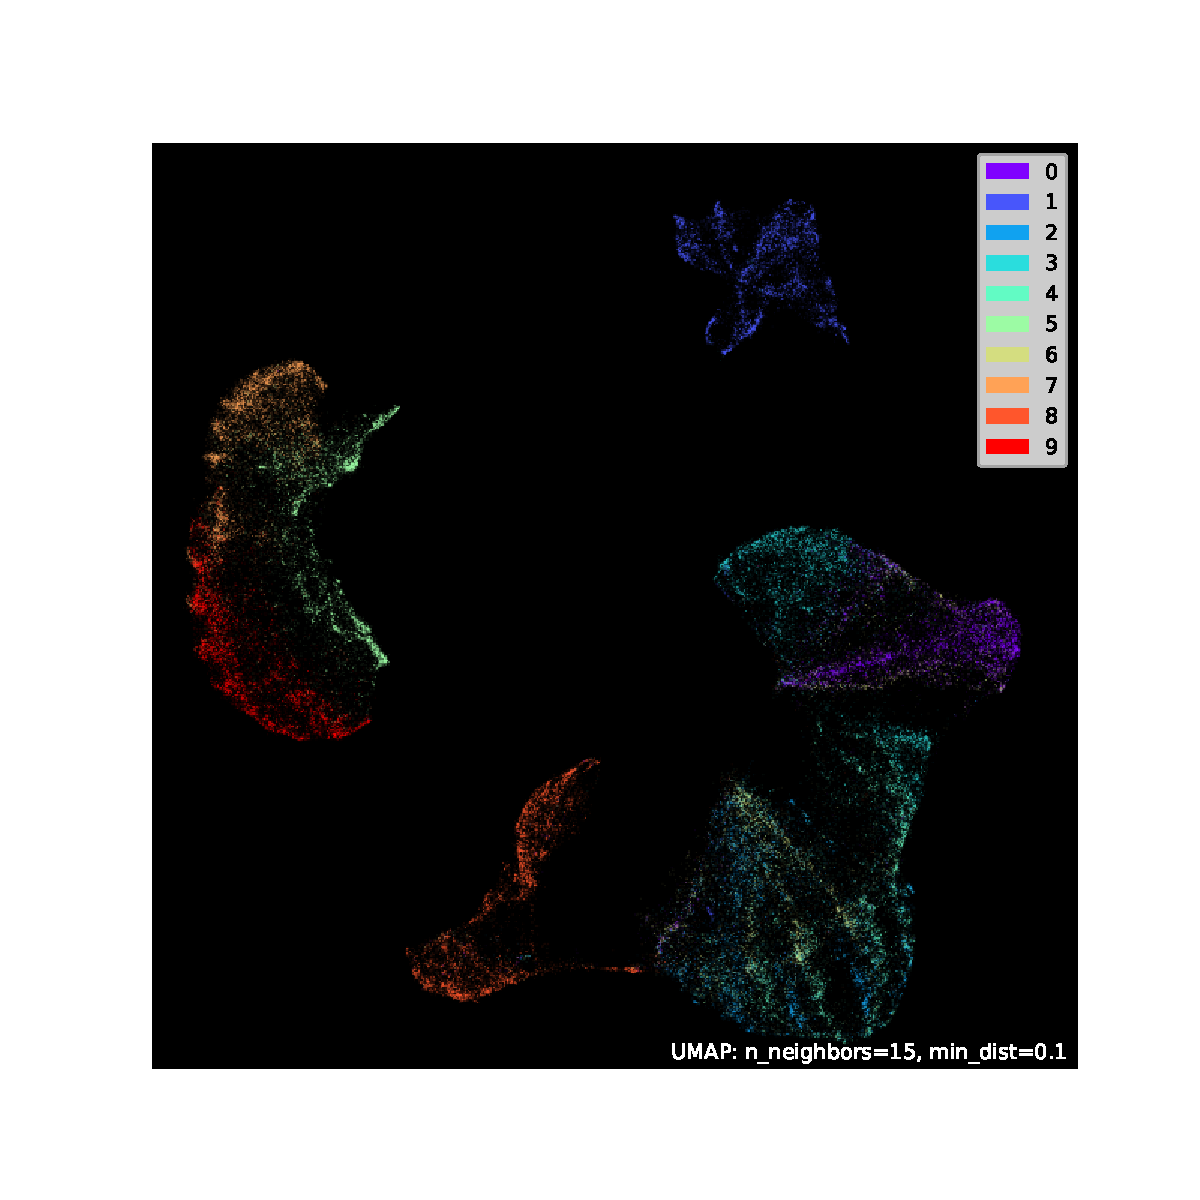
\includegraphics[width=12cm, height=10cm]{fmnist.pdf}
  \caption{Result of UMAP on the much larger Fashion-MNIST dataset.}
  \label{fig:fmnist}
\end{figure}

It intuitively makes sense to see that shoes should be generally projected close to each other, as we see with sneakers, sandals and ankle boots. Trousers are found in the top-left corner, isolated from the rest. In the \textit{UMAP examples} notebook, we also provide an interactive version of the resulting projection on a subset of Fashion-MNIST, allowing the user to see the labels of individual points upon zooming.

An interesting property that UMAP allows us to study is the connectivity of the topological representation of the original high-dimensional data. This can be useful for diagnostic purposes, but in the case of this text, it corresponds to studying the connected components. It should be noted that computing and plotting the connectivity of the dataset can be rather expensive, so it is recommended to check subsamples instead. We can see examples of it on \ref{fig:fmnist_connectivity} and \ref{fig:fmnist_connectivity_hammer}.

\begin{figure}[h!]
  \centering
  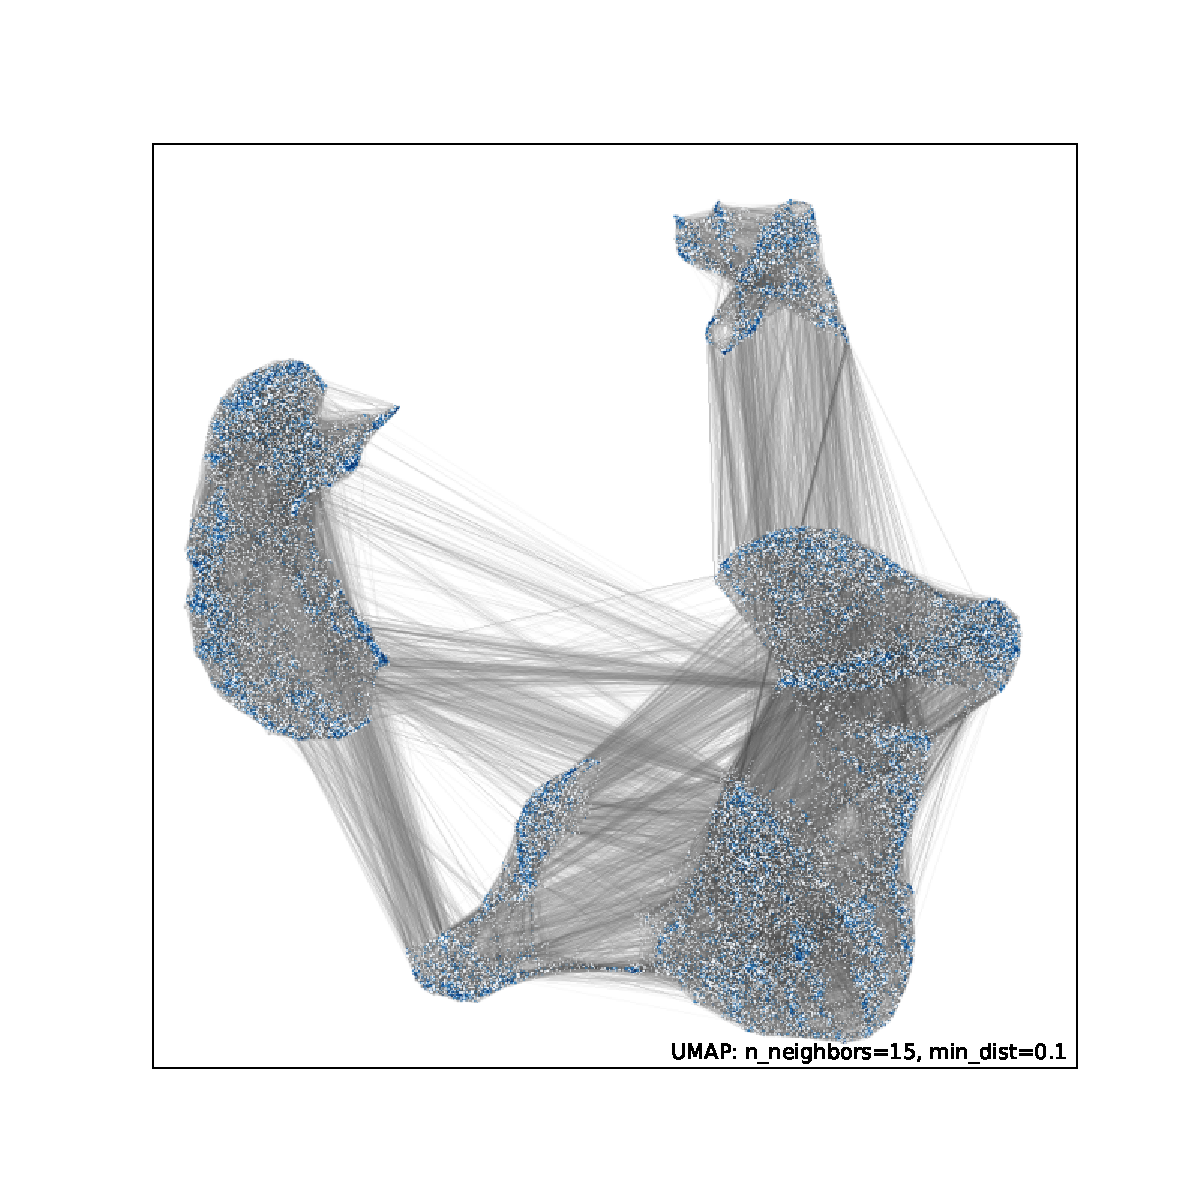
\includegraphics[width=12cm, height=10cm]{fmnist_connectivity.pdf}
  \caption{Points of connectivity of Fashion-MNIST.}
  \label{fig:fmnist_connectivity}
\end{figure}

\begin{figure}[h!]
  \centering
  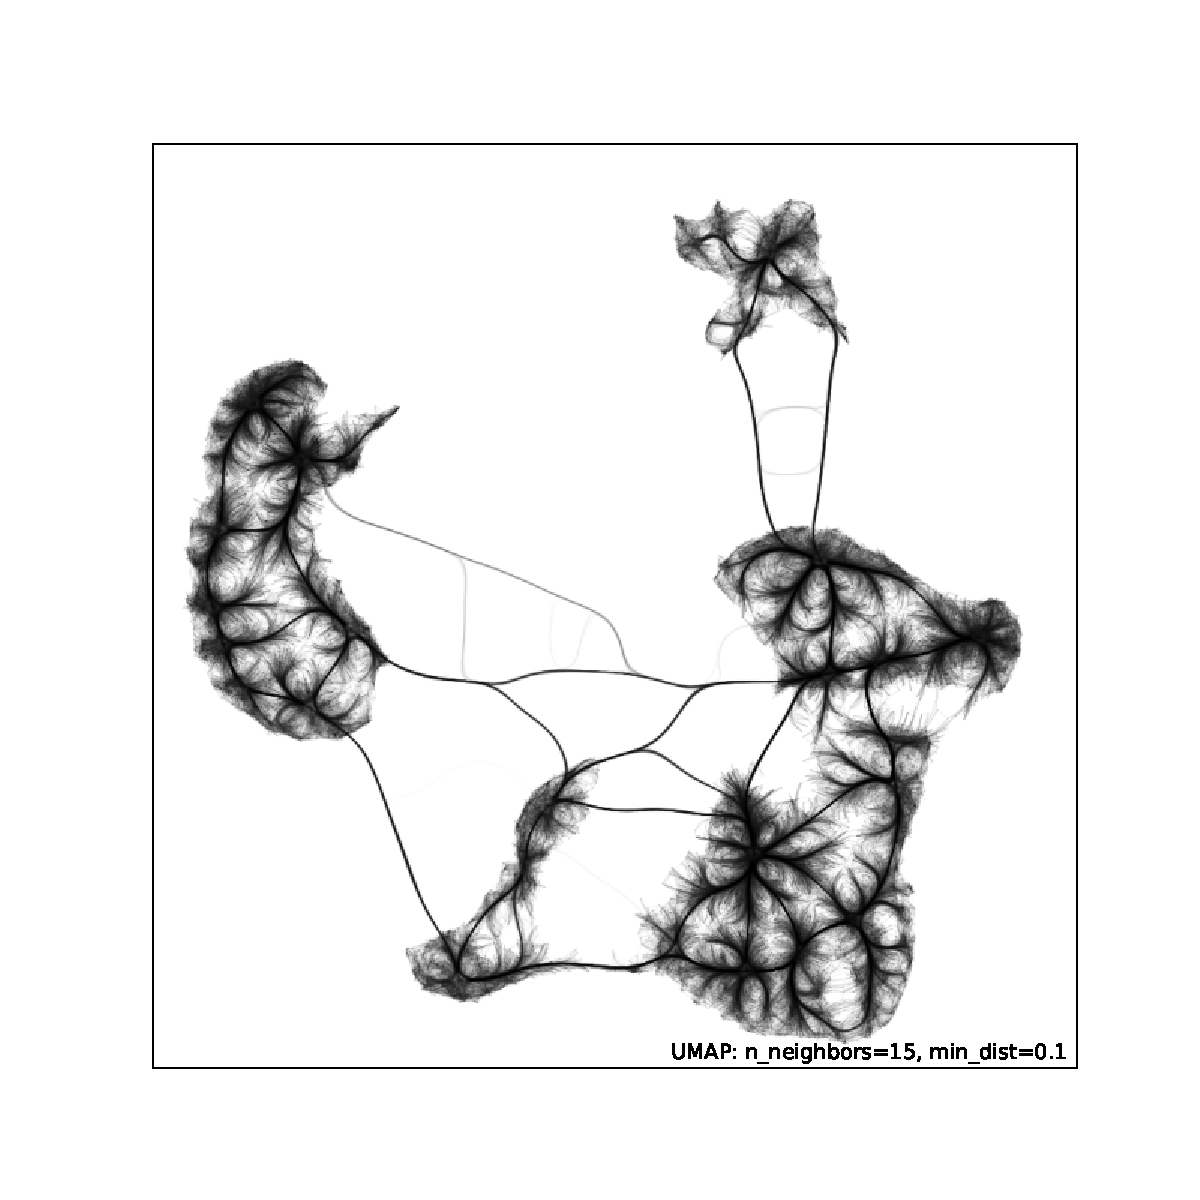
\includegraphics[width=12cm, height=10cm]{fmnist_connectivity_hammer.pdf}
  \caption{A less busy view of connectivity of Fashion-MNIST.}
  \label{fig:fmnist_connectivity_hammer}
\end{figure}

\section{Mapper}
As was mentioned in the beginning of this text, the methods of persistence topology can become computationally infeasible for larger datasets, making them practically unusable for datasets with measurements in the counts of millions and above. This was seen in the rapidly-growing number of simplices in the Vietoris-Rips complex. Furthermore, interpreting the output of persistence homology for high-dimensional data can be difficult to interpret (what does the presence of a 1-dimensional loop in a 50-dimensional space indicate?). One approach to tackle this issue is to combine persistence with clustering, resulting in the Mapper algorithm that we're going to discuss.

We're going to introduce the multiscale clustering method of Singh, Mémoli and Carlsson \cite{singh2007topological}. Let's assume that the data is presented as a finite metric space $(P, d)$. Let us then choose:

\begin{itemize}
  \item a \textit{filter function} $f: P \to \mathbb{R}^{n}$
  \item a cover $\mathcal{C} = \{U_{\alpha}\}$ of the range of $f$ in $\mathbb{R}^{n}$
\end{itemize}
The cover is typically taken to be a collection of overlapping cubes. In $\mathbb{R}$, we would be looking at a collection of closed intervals. Software packages will want you to specify the number of covering intervals and the percentage of overlap you allow. We then proceed with the algorithms as follows:

\begin{enumerate}
  \item Cluster each inverse image $f^{-1}(U_{\alpha}) \subseteq P$, regarded as a metric subspace of $P$, for all $U_{\alpha} \in \mathcal{C}$. Denote by $C_{\alpha, i}$ the i-th cluster. Here, a point can appear in multiple nodes due to the overlap.

  \item Form a graph where the vertices are given by the clusters $C_{\alpha, i}$ as $\alpha$ and $i$ vary and there is an edge between $C_{\alpha, i}$ and $C_{\alpha', j}$ when
        \begin{equation*}
          C_{\alpha, i} \cap C_{\alpha', j} \neq \varnothing
        \end{equation*}

  \item Assign a color to each vertex in the graph corresponding to a particular cluster $C_{\alpha, i}$ according to the average value of $f$ on $x \in C_{\alpha, i}$.
\end{enumerate}

Mapper's strength lies in the flexibility of choices we can make during the creation of the graph. For the projection, we can take any projection method from mathematics, statistics, machine learning or  econometrics -- PCA, t-SNE, UMAP, even something as simple as projecting on the $x-$axis.

The same applies for the choice of clustering algorithms. We can pick any method -- hierarchical, density-based and any distance metric. The distance metric does not need to satisfy the triangle inequality, giving us the option to choose from the wider range of similarity metrics like the Kullback-Leibler divergence and so on.

Because Mapper is primarily a visual tool, most software packages include additional tooling to improve upon the basic algorithm and help with further exploration. That may involve a combination of the following:

\begin{itemize}
  \item Size the nodes by a function of interest (number of members inside the cluster, etc.)
  \item Color the nodes by a function of interest (average spendings, number of purchases, etc.)
  \item Shape the nodes given some condition (circles for group 1, squares for group 2, etc.)
  \item Size the graph edges by a function of interest (number of overlapping cluster members, etc.)
  \item Color the graph edges by a function of interest (average color of connected nodes, etc.)
  \item Shape the graph edges given a condition (dotted lines for group 1, solid line elsewhere, etc.)
  \item Descriptive statistics on the nodes and the graph
\end{itemize}

All in all, this makes Mapper one of the most flexible approaches to dataset visualizations, giving the user the option the construct the final graph exactly the way they intended. For the Mapper examples, we will make use of the Python libraries \textit{scikit-tda} \cite{scikittda2019} and \textit{giotto-tda} \cite{tauzin2020giottotda}.

We can start with simple, synthetic examples before moving onto real data to see what the results of Mapper are and how they differ when we change the parameters or used methods.

\subsection{Toy examples}
We will start by generating 5000 points sampled from two nested circles in the plane with some added Gaussian noise. We can see the plotted dataset in \ref{fig:mapper_circles}. In our first attempt, we will project our data onto the $x-$ and $y-$axes, choose 10 covering intervals with a 30\% overlap and use the DBSCAN clustering algorithm.

In figure \ref{fig:mapper_circles_graph} we can see that Mapper succesfuly captured the salient features - those being the two holes in the nested circles. The coloring of the node used the default settings of \textit{giotto-tda} -- coloring the nodes by the average row index of the data in the cluster; with 5000 generated points, we thus have 5000 rows. The node size here is given by the number of data points in the node.

\begin{figure}[h!]
  \centering
  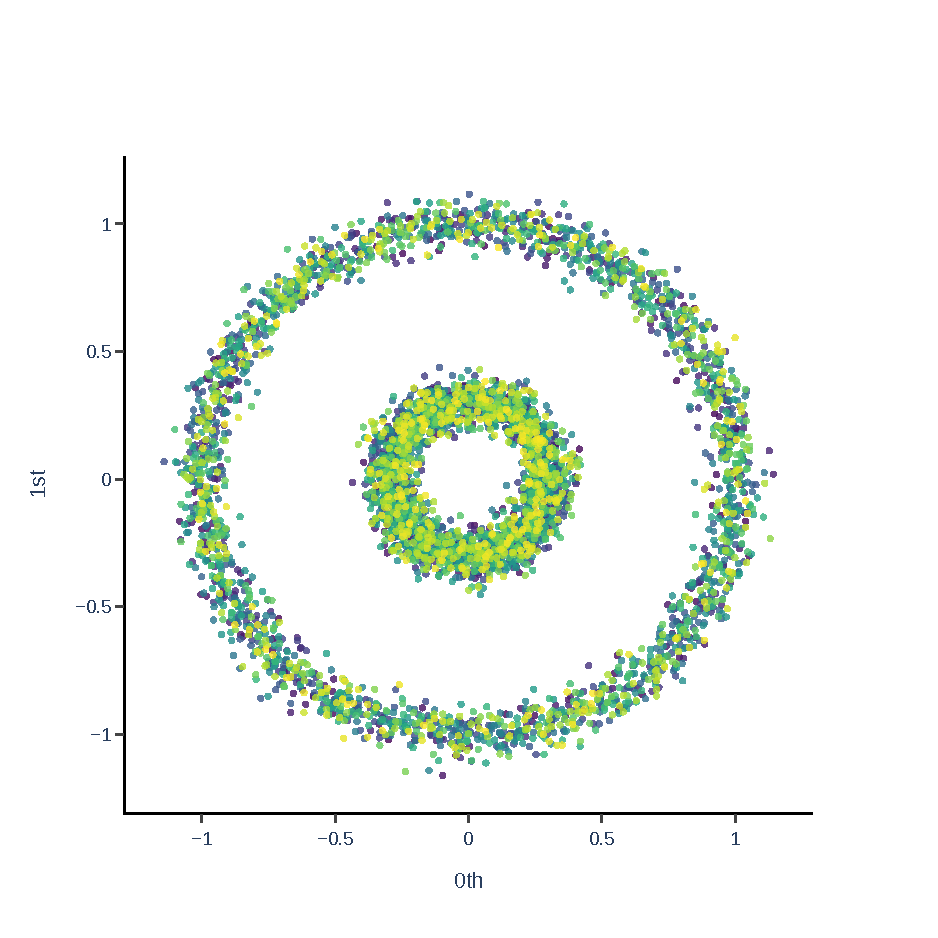
\includegraphics[width=10cm, height=10cm]{mapper_circles.pdf}
  \caption{Our toy example for now - two nested circles.}
  \label{fig:mapper_circles}
\end{figure}

\begin{figure}[h!]
  \centering
  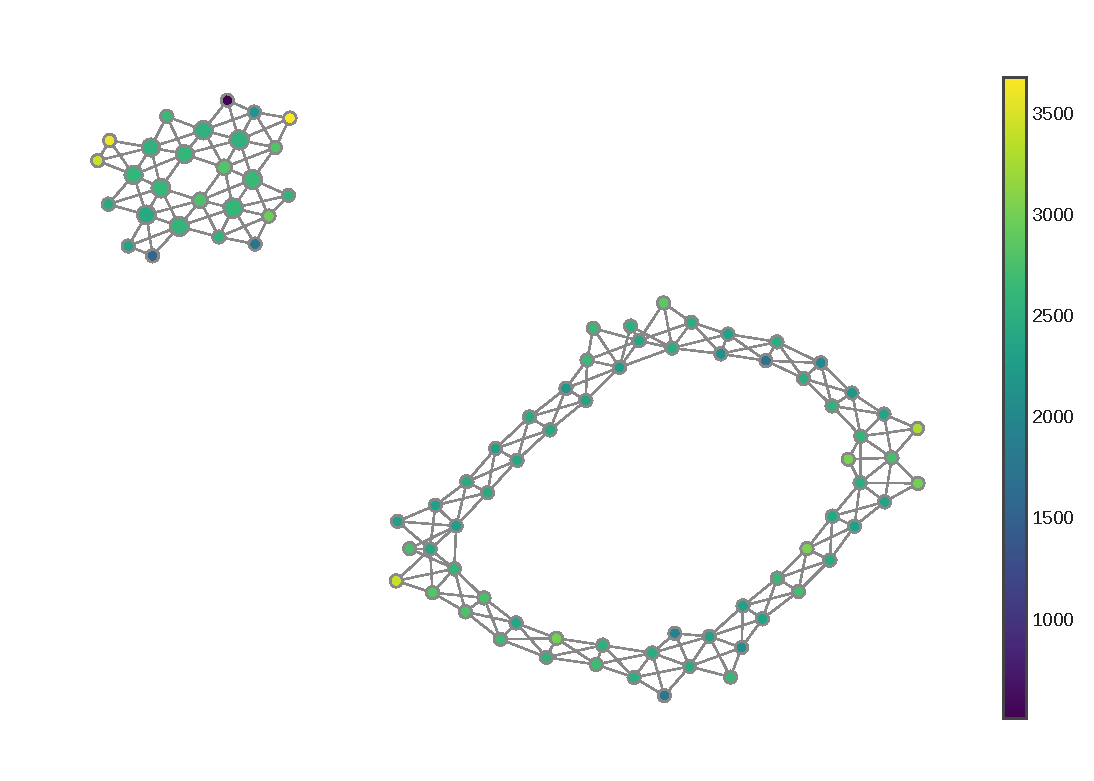
\includegraphics[width=10cm, height=10cm]{mapper_circles_graph.pdf}
  \caption{First result of applying Mapper.}
  \label{fig:mapper_circles_graph}
\end{figure}

The coloring or the size do not convey any particularly interesting information in this case; here we were more interested to recover the presence of the two underlying holes. On the other hand, coloring by the average value of the $x-$ or $y-$coordinates would be more instructive, as revealed on \ref{fig:mapper_circles_coordinates}. Here we see that the $x-$coordinates of the inner circle, closer to the origin, are colored in such a way that lies near the $0$ point of the spectrum. We would see a similar, but flipped, version of the coloring had we used the $y$-coordinates instead.

\begin{figure}[h!]
  \centering
  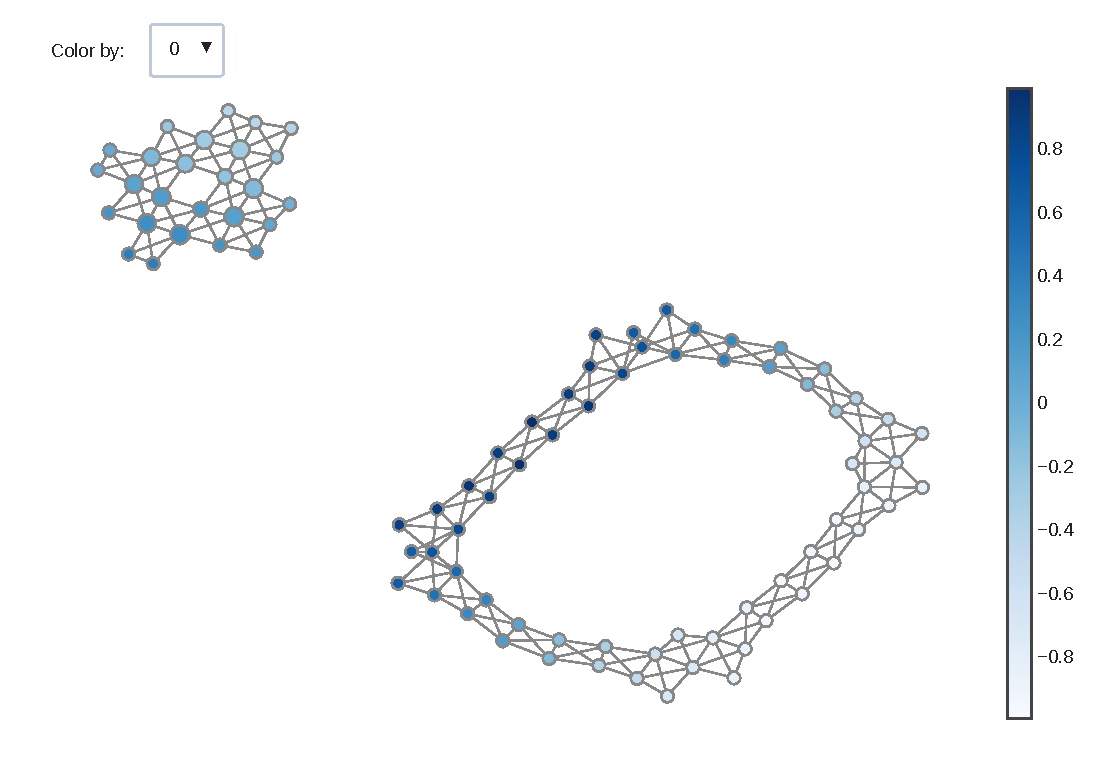
\includegraphics[width=10cm, height=10cm]{mapper_circles_coordinates.pdf}
  \caption{Nodes colored by the average $x$-coordinate.}
  \label{fig:mapper_circles_coordinates}
\end{figure}

We can, if we want to, color by something like the first principal component of PCA, as seen in \ref{fig:mapper_circles_pca}. In this context, it doesn't reveal anything particularly interesting but it may be more useful in applications where PCA is actively used.

\begin{figure}[h!]
  \centering
  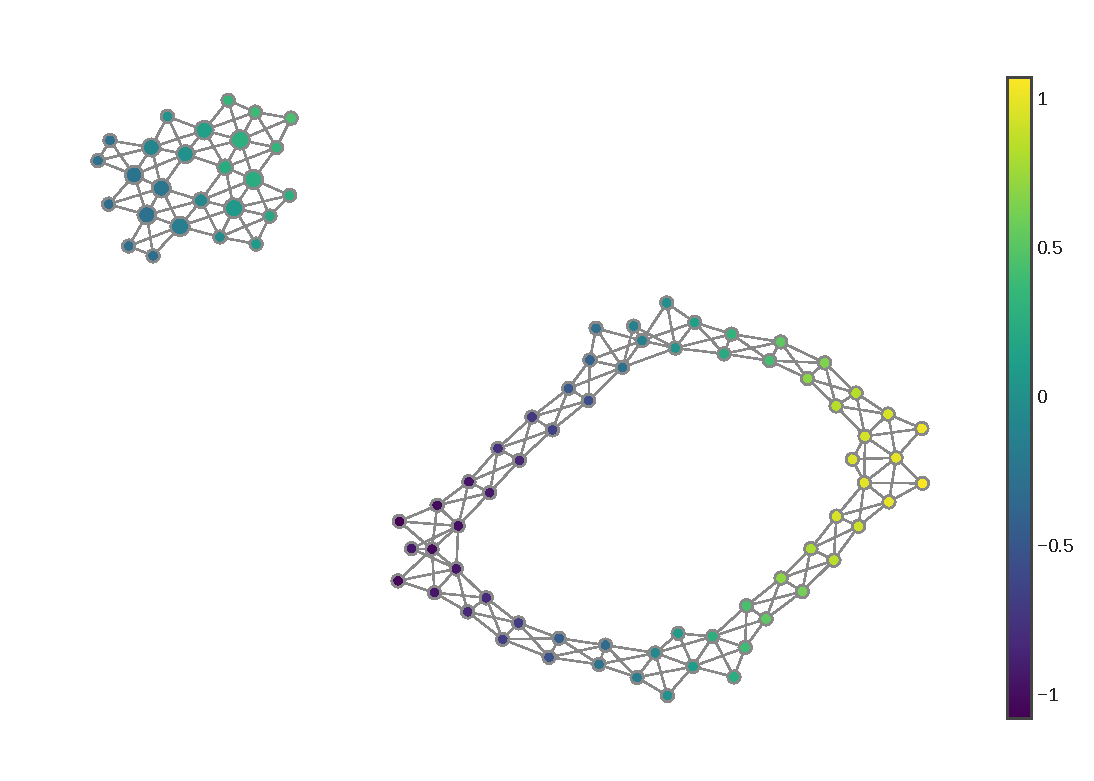
\includegraphics[width=10cm, height=10cm]{mapper_circles_pca.pdf}
  \caption{Nodes colored by the average first PCA component.}
  \label{fig:mapper_circles_pca}
\end{figure}

As mentioned above, we can colord by proportions of some categorical variable -- one that is either already present or one that we create. Let us try to separate the inner and outer circle more cleanly. We can add a categorical column to the dataframe, with a value of ``A'' for the outer circle and ``B'' for the inner circle, where the testing criterium is whether
\begin{equation*}
  x^{2} + y^{2} < \frac{1}{4}.
\end{equation*}

The result of this can be seen on \ref{fig:mapper_circles_groups}, where the inner and outer circle are now exactly separated. As with the coordinates, we would see a flipped version of this graph for group ``B''. It should also be noted that the color spectrum only attains two values -- $\{0, 1\}$.

\begin{figure}[h!]
  \centering
  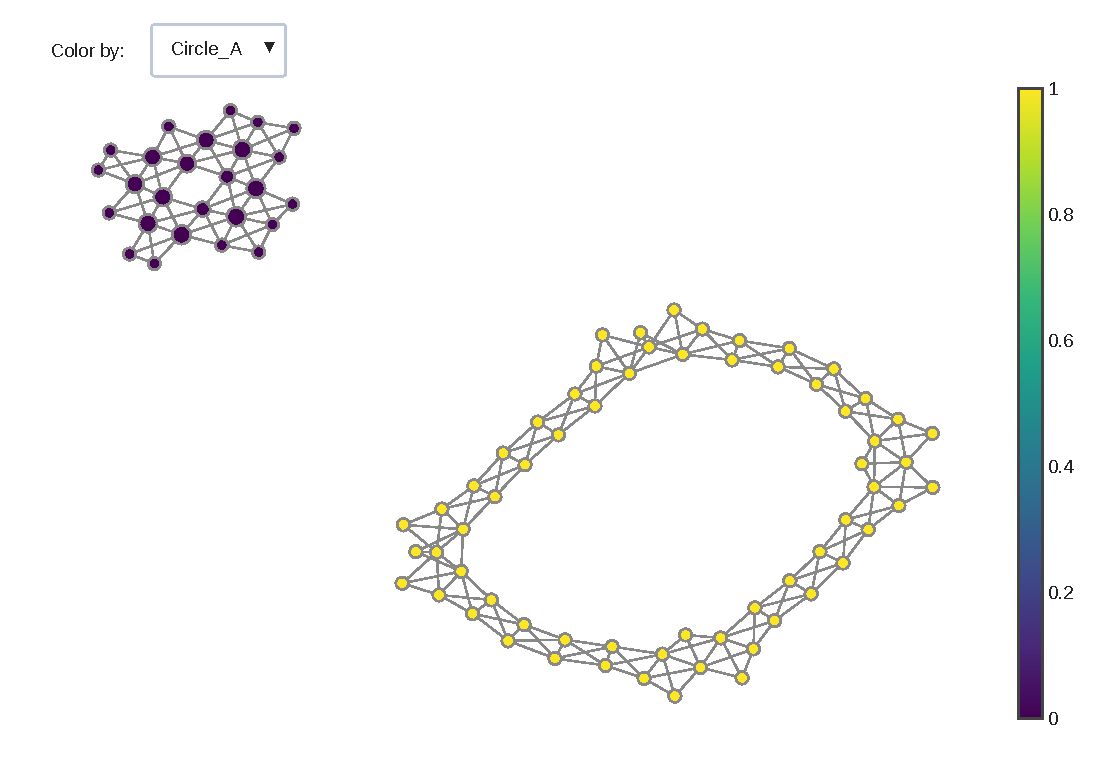
\includegraphics[width=10cm, height=10cm]{mapper_circles_groups.pdf}
  \caption{Nodes colored by categorical variables.}
  \label{fig:mapper_circles_groups}
\end{figure}

Finally, we can take a look and compare what happens when we use a different filtration function on the dataset. For example, we could project by taking the sum of the $(x,y)$ coordinates. This results in \ref{fig:mapper_circles_sum}.

\begin{figure}[h!]
  \centering
  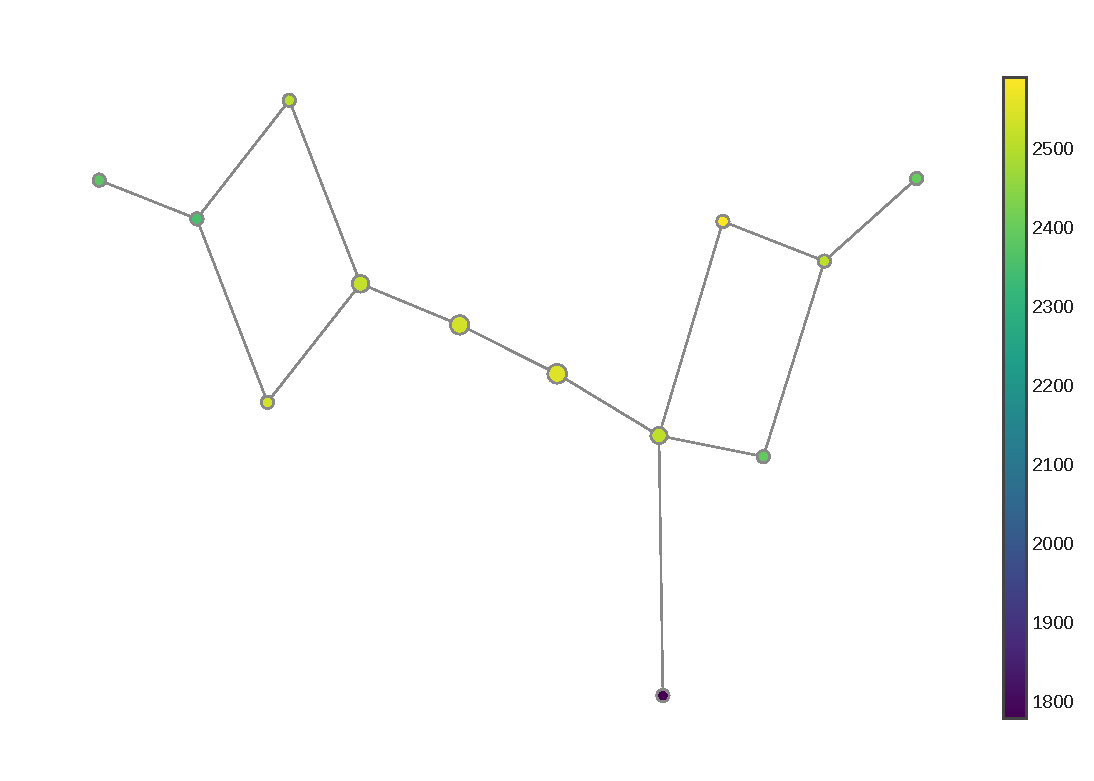
\includegraphics[width=12cm, height=10cm]{mapper_circles_sum.pdf}
  \caption{The effect of a different filtration function; in this case, the sum of the individual coordinates.}
  \label{fig:mapper_circles_sum}
\end{figure}

The presence of the two loops was still properly encoded, although this time we don't have the same level of separation as we did by projecting on the individual coordinates.

\subsection{Stock market data}
We can now take a look at how one could potentially use Mapper to improve your analysis of stock market data. Specifically, we will look at the closing prices of the SP500 index companies, starting from 01.01.2024 up to 01.01.2025. The choice of date is arbitrary and one could easily choose a much larger time interval to consider, but for the sake of this example, one year will suffice. The data was fetched from Yahoo Finance through their API and stored in a dataframe. A simple indicator of interest when dealing with stock market data is the log-return of the stock price. As such, our first filtration function will be the log-percent return after the data is normalized.

Our goal here will be to cluster the company tickers in a way that similar behaviour of the stock value is represented in similar tickers sharing the same cluster. We could take the transpose of our dataset instead and try to cluster the 252 trading days of the year. This could perhaps be useful if we wanted to analyze which days or periods of the year showed significant drops or increase in the SP500 index. We could then correlate the clusters with geopolitical events such as the US presidential election, which brought an increase in stock prices for large tech companies, for example.

After normalizing the dataset, we first reduced the dimension to 150 via the Isomap algorithm before using UMAP to reduce it to 2. Our clustering algorithm of choice here was DBSCAN with the cosine metric. Using \textit{scikit-tda}, the result is stored in a \textit{html} file that you can open in your web browser. All the files for this section can be located in the \textit{figures/} folder. Our first view can be seen on \ref{fig:mapper_log_return}.

\begin{figure}[h!]
  \centering
  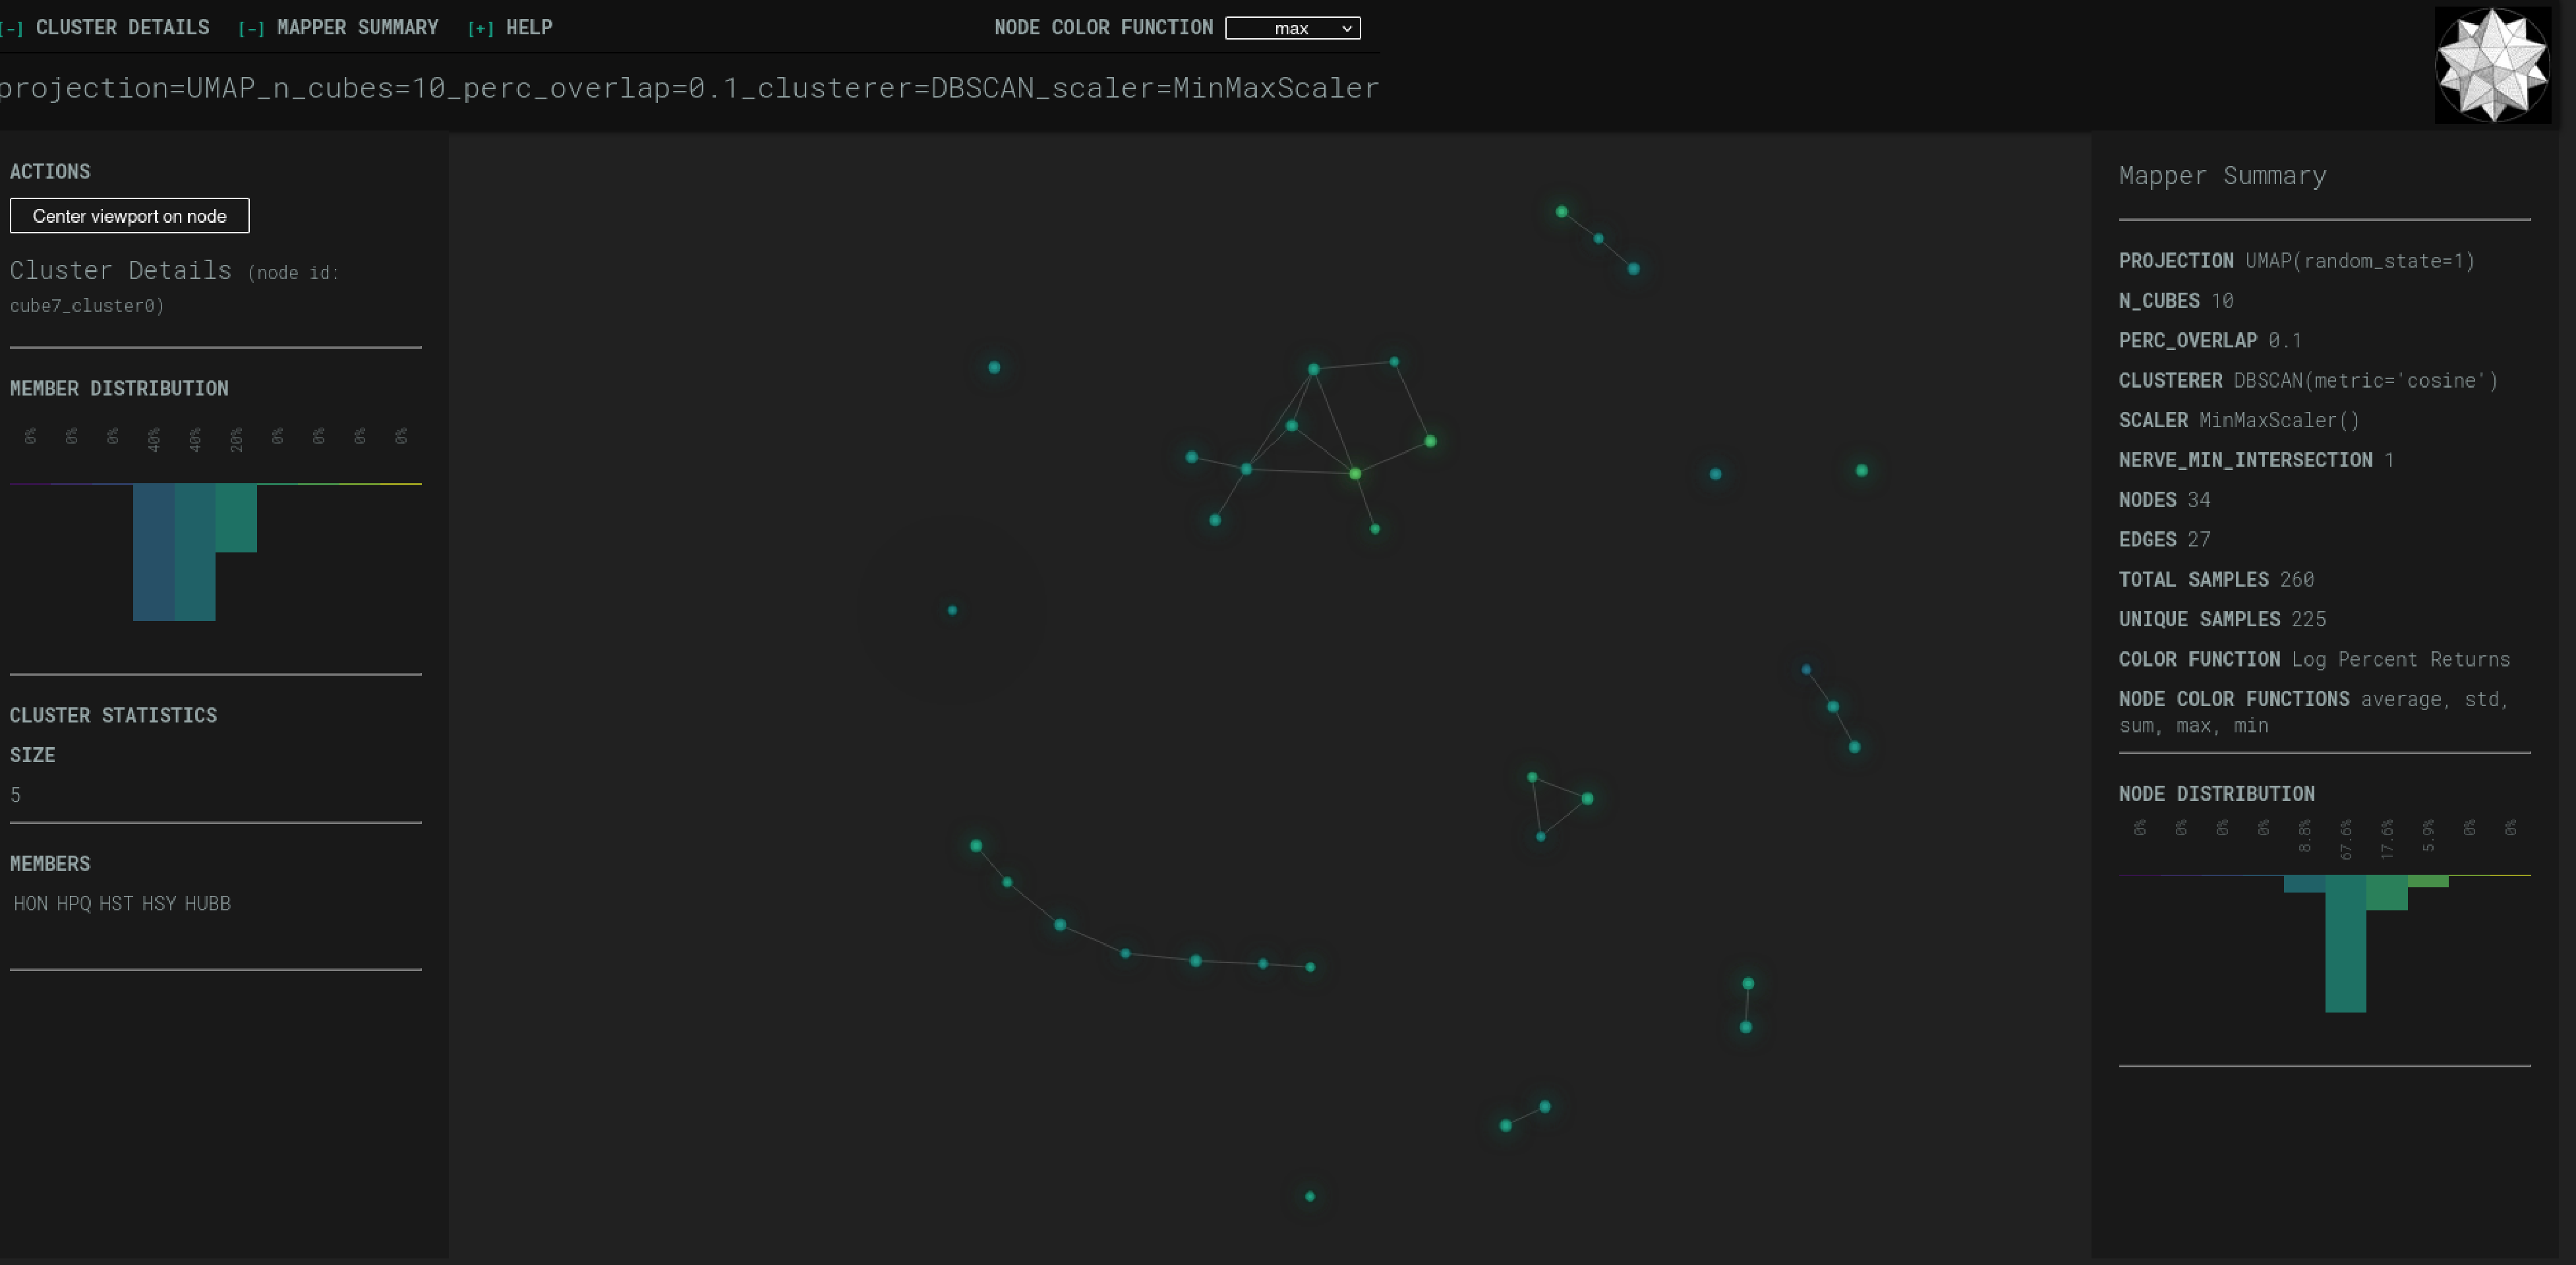
\includegraphics[width=15cm, height=12cm]{Mapper_log_return_example.pdf}
  \caption{View of the Mapper clustering summary with \textit{scikit-tda}.}
  \label{fig:mapper_log_return}
\end{figure}

We interpret the results as follows -- given that our color function is the log-percent return of the individual tickers, the clusters correspond to tickers who share a similar trading profile between each other. That is, underperformers would have darker colors, while companies that performed exceptionally well would be on the brighter end of the spectrum. In the graph \ref{fig:mapper_log_return}, we added multiple cluster coloring rules to compare. As mentioned previously, the default strategy is to color the final cluster by the average of the nodes inside. Here, we can also color by the average, maximum, minimum, the sum of the standard deviation. The only interesting results are when we look at the minimum and maximum log-percent returns of the clusters. While we have some stocks that performed better than the rest, most companies had a similar run during that one year. One could anticipate greater differences had we considered the closing prices over multiple years instead.

We could also choose a different color function, such as the volatility of the underlying stock. The notion of volatility we will look at is quite crude -- we simply take the standard deviation of the stock prices over the 252 days. Stock traders and market specialists would throttle us for this gross simplification, which is why we ignore their opinions and continue. The different color function drastically changes the resulting graph, as seen in \ref{fig:mapper_volatility}.

\begin{figure}[h!]
  \centering
  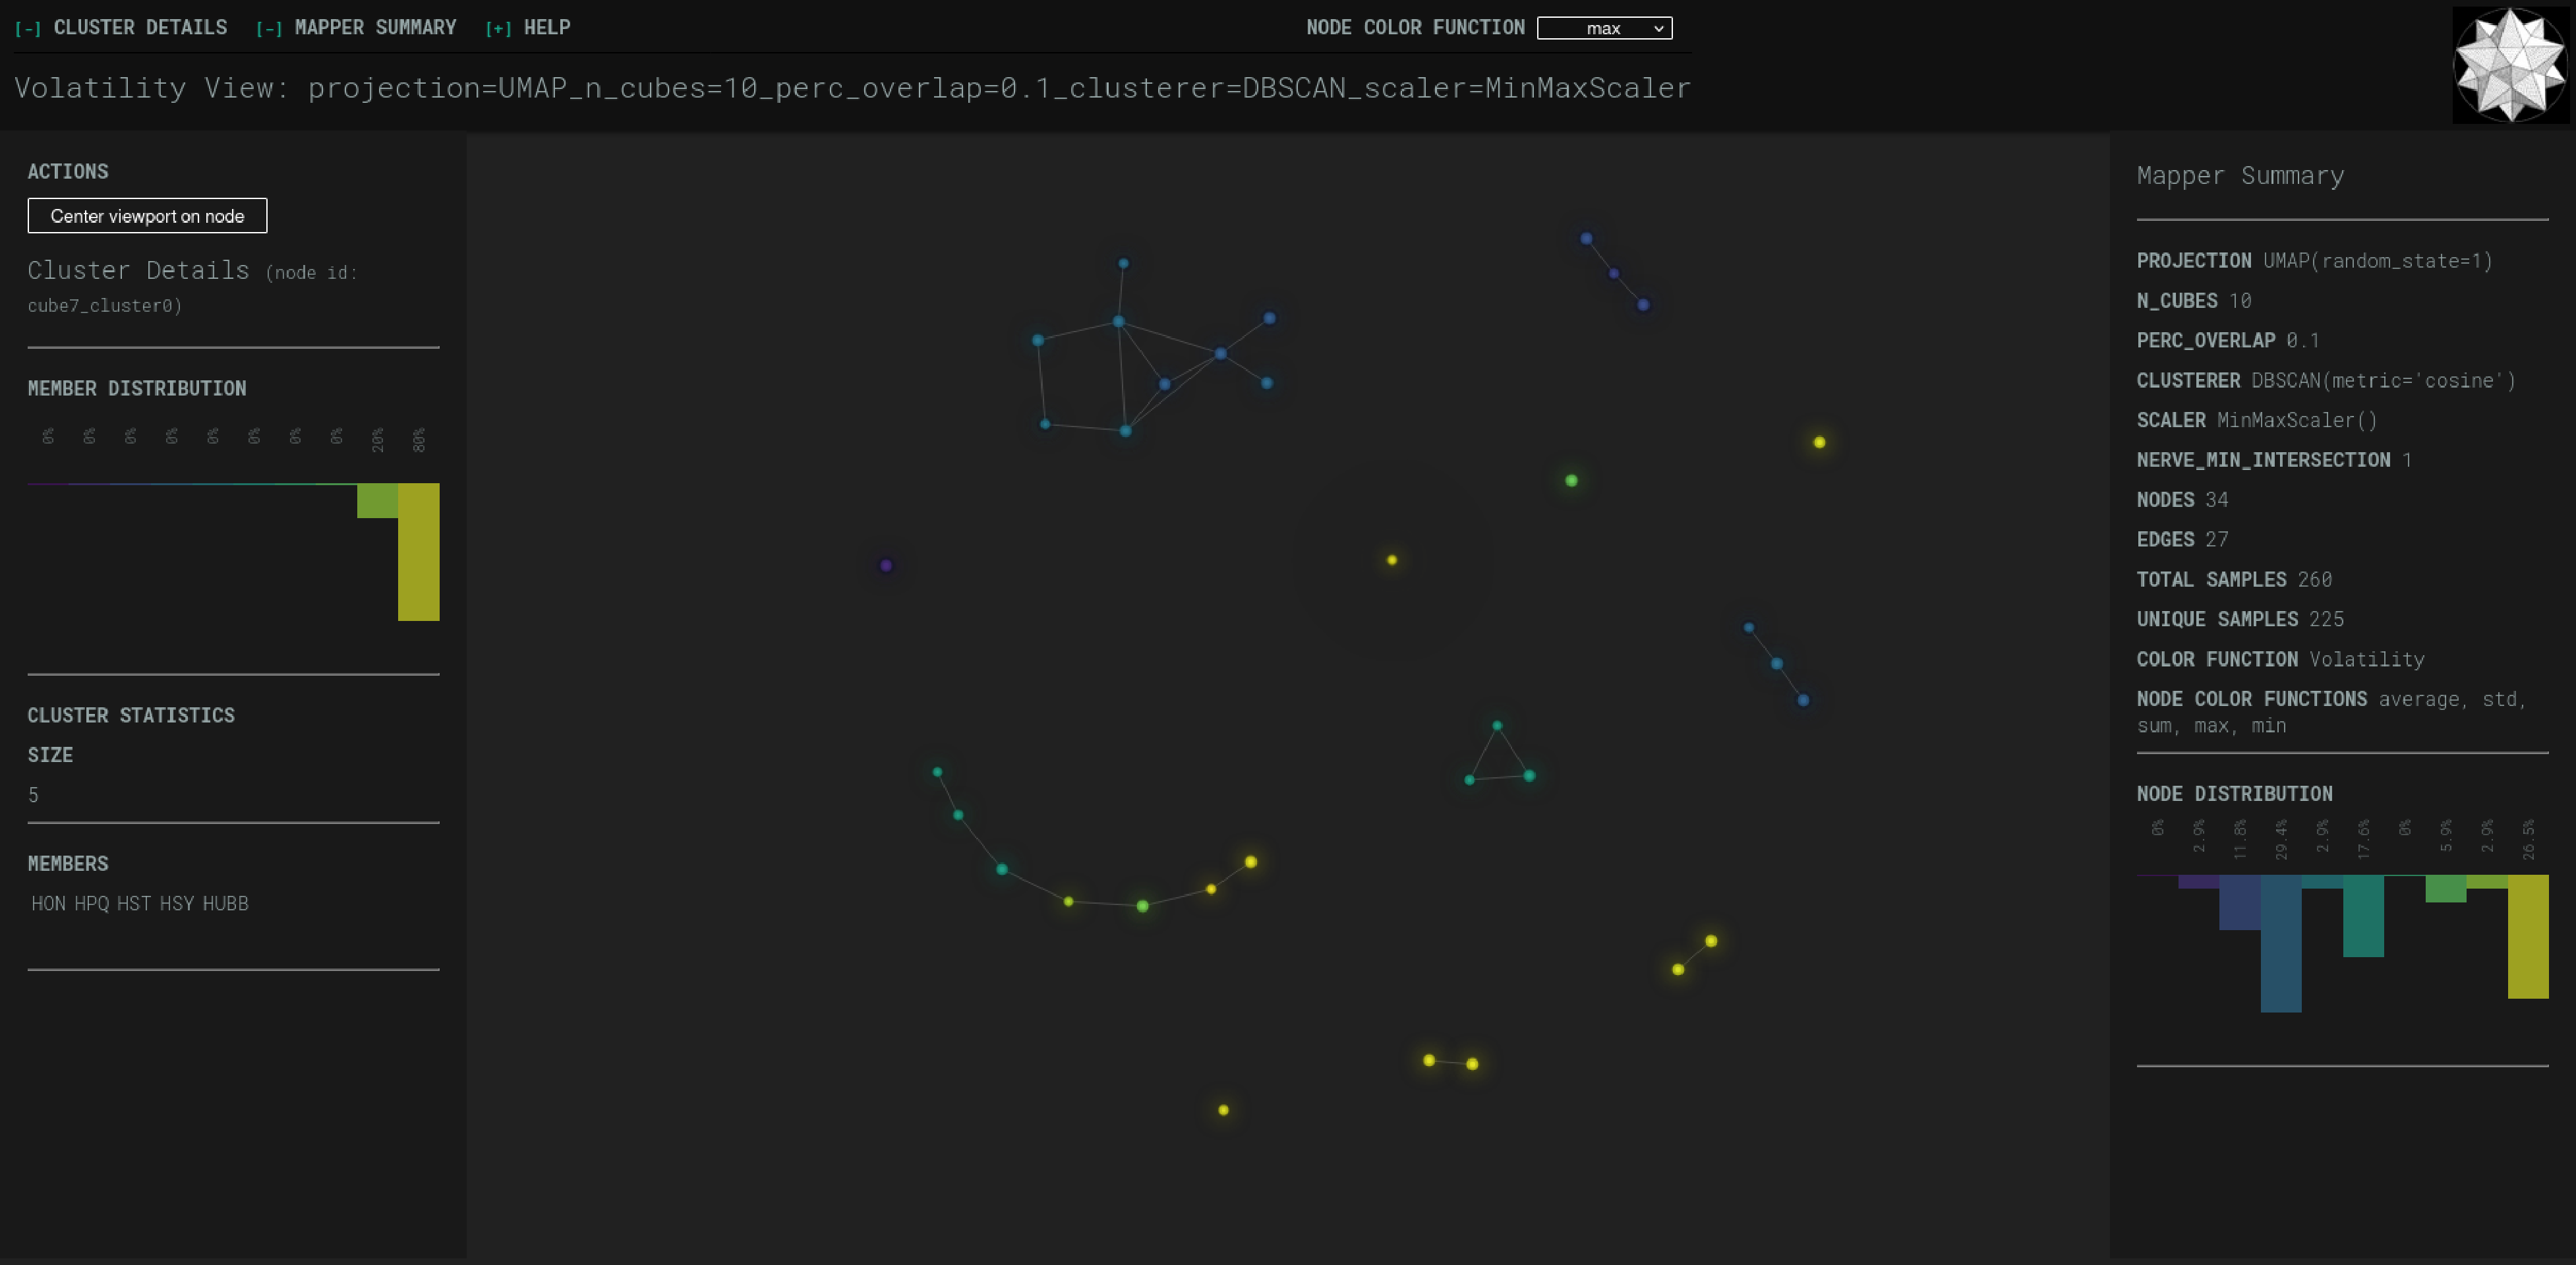
\includegraphics[width=15cm, height=12cm]{Mapper_volatility.pdf}
  \caption{Mapper graph of the SP500 data with the color function being the volatility of the stock.}
  \label{fig:mapper_volatility}
\end{figure}

Here we use the maximum of the volatility to color the resulting clusters, looking for stocks with an unusually high variance in the closing prices. Already, we can see that we have more outliers on both ends of the color spectrum, compared to the log-percent return. The benefit of the Mapper implementation in \textit{scikit-tda} is that it allows us to see directly which SP500 tickers are in the clusters by simply hovering over them. It also gives us the cluster ID, allowing us to plot the cluster data separatly from the rest. This way, we can plot the dark purple cluster, suggesting the lowest maximal volatility of closing prices in \ref{fig:mapper_volatility_low}.

\begin{figure}[h!]
  \centering
  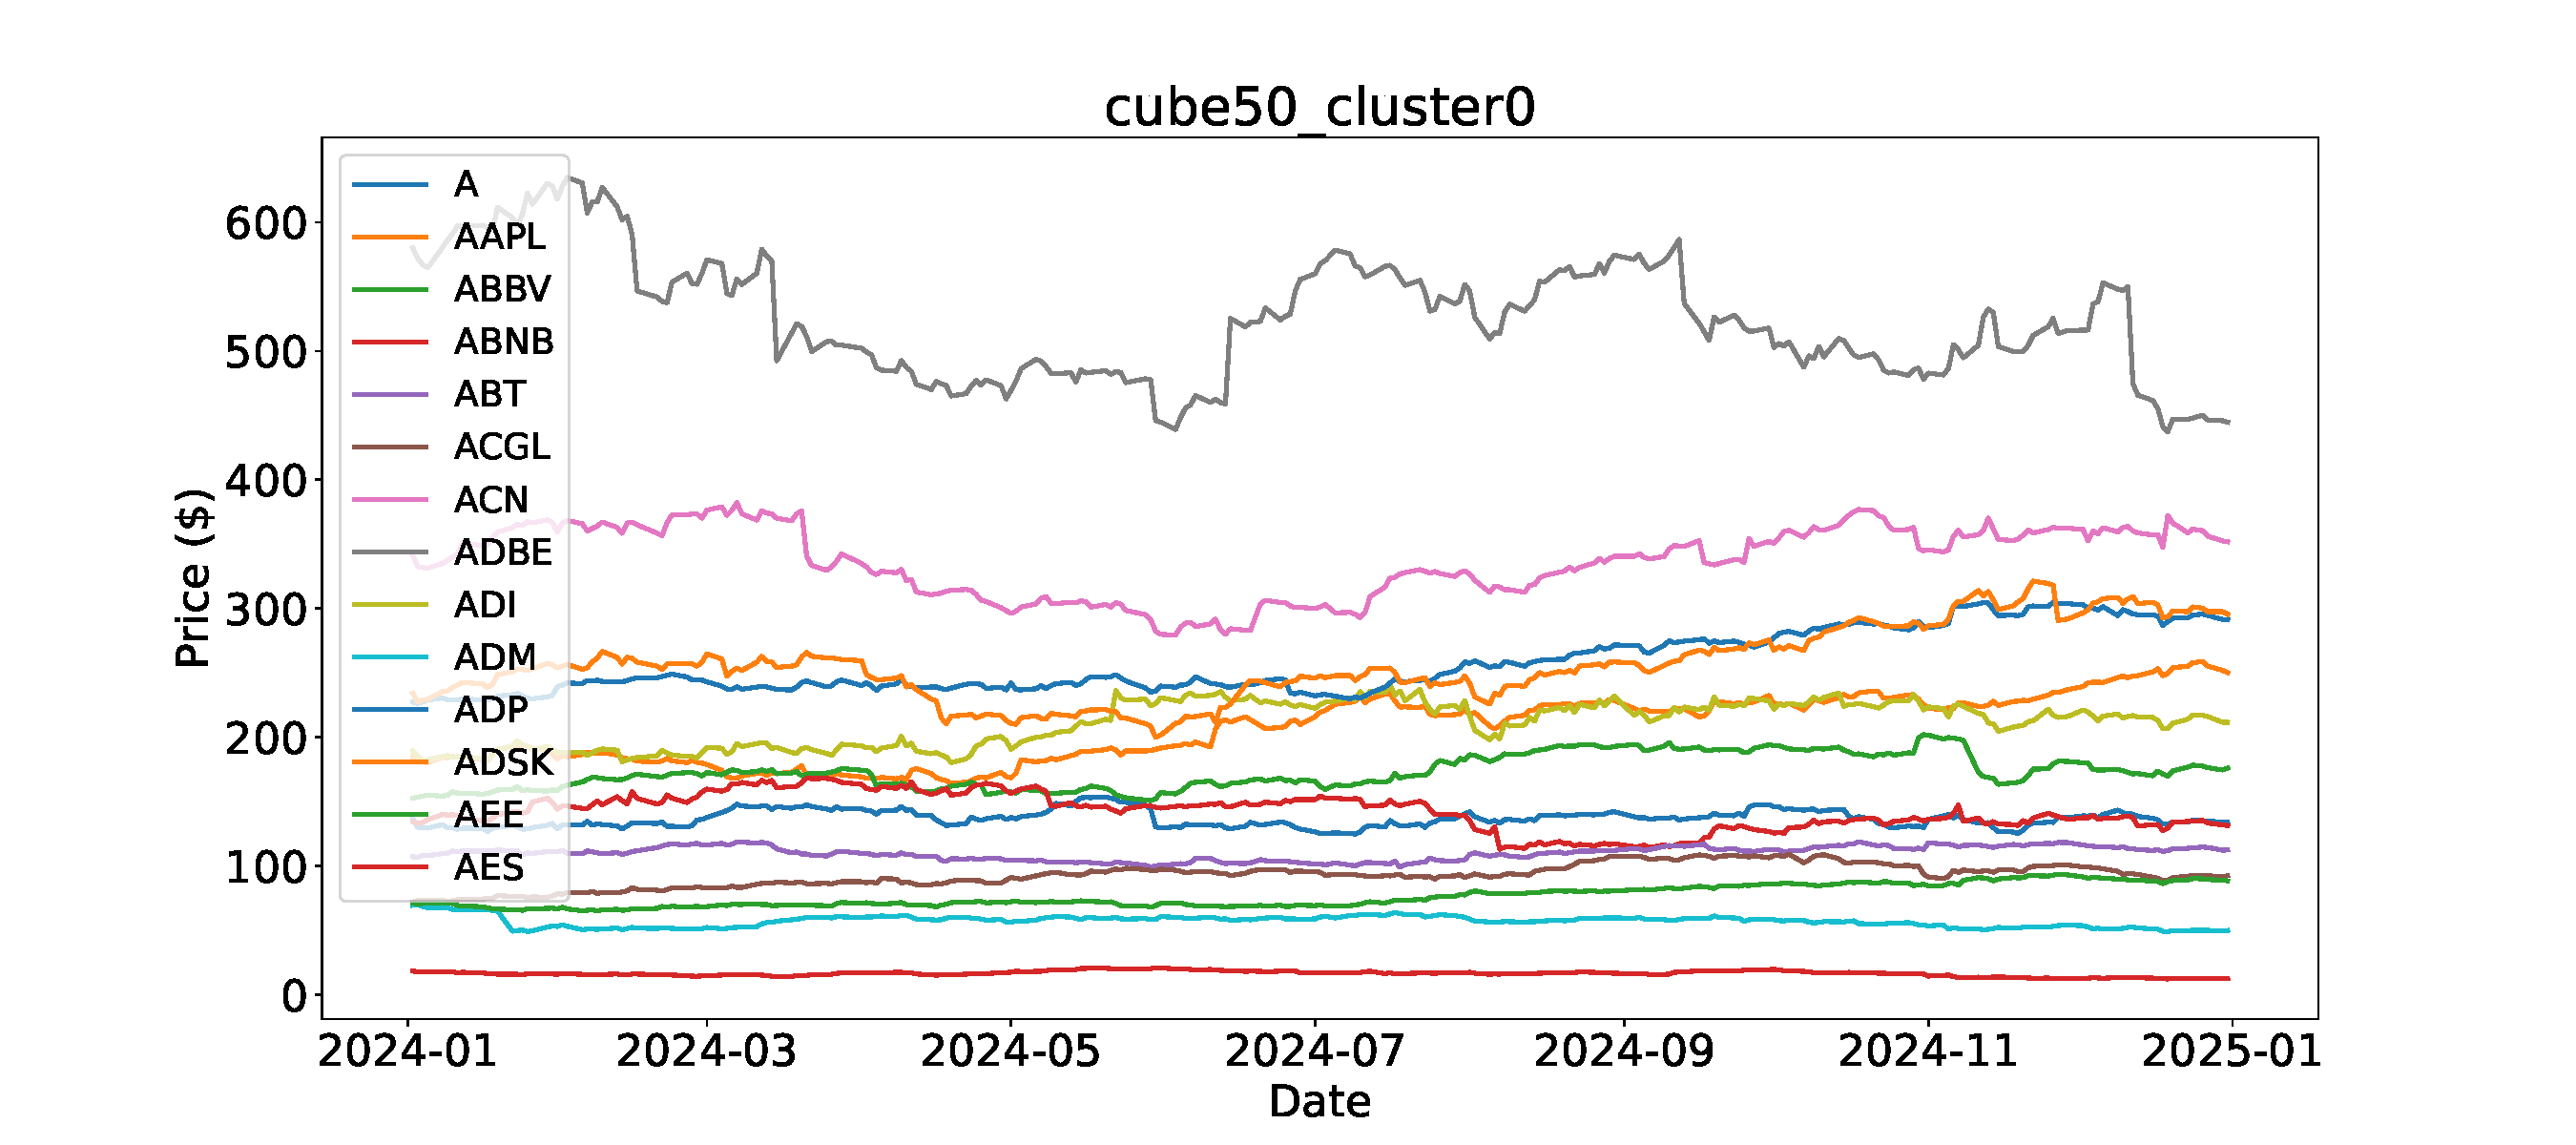
\includegraphics[width=14cm, height=10cm]{mapper_volatility_low_projection=UMAP_n_cubes=10_perc_overlap=0.1_clusterer=DBSCAN_scaler=MinMaxScaler.pdf}
  \caption{Cluster of tickers with the lowest maximal volatility.}
  \label{fig:mapper_volatility_low}
\end{figure}

We can contrast it with the bright yellow clusters, the ones with the highest maximal volatility, in \ref{fig:mapper_volatility_high}.

\begin{figure}[h!]
  \centering
  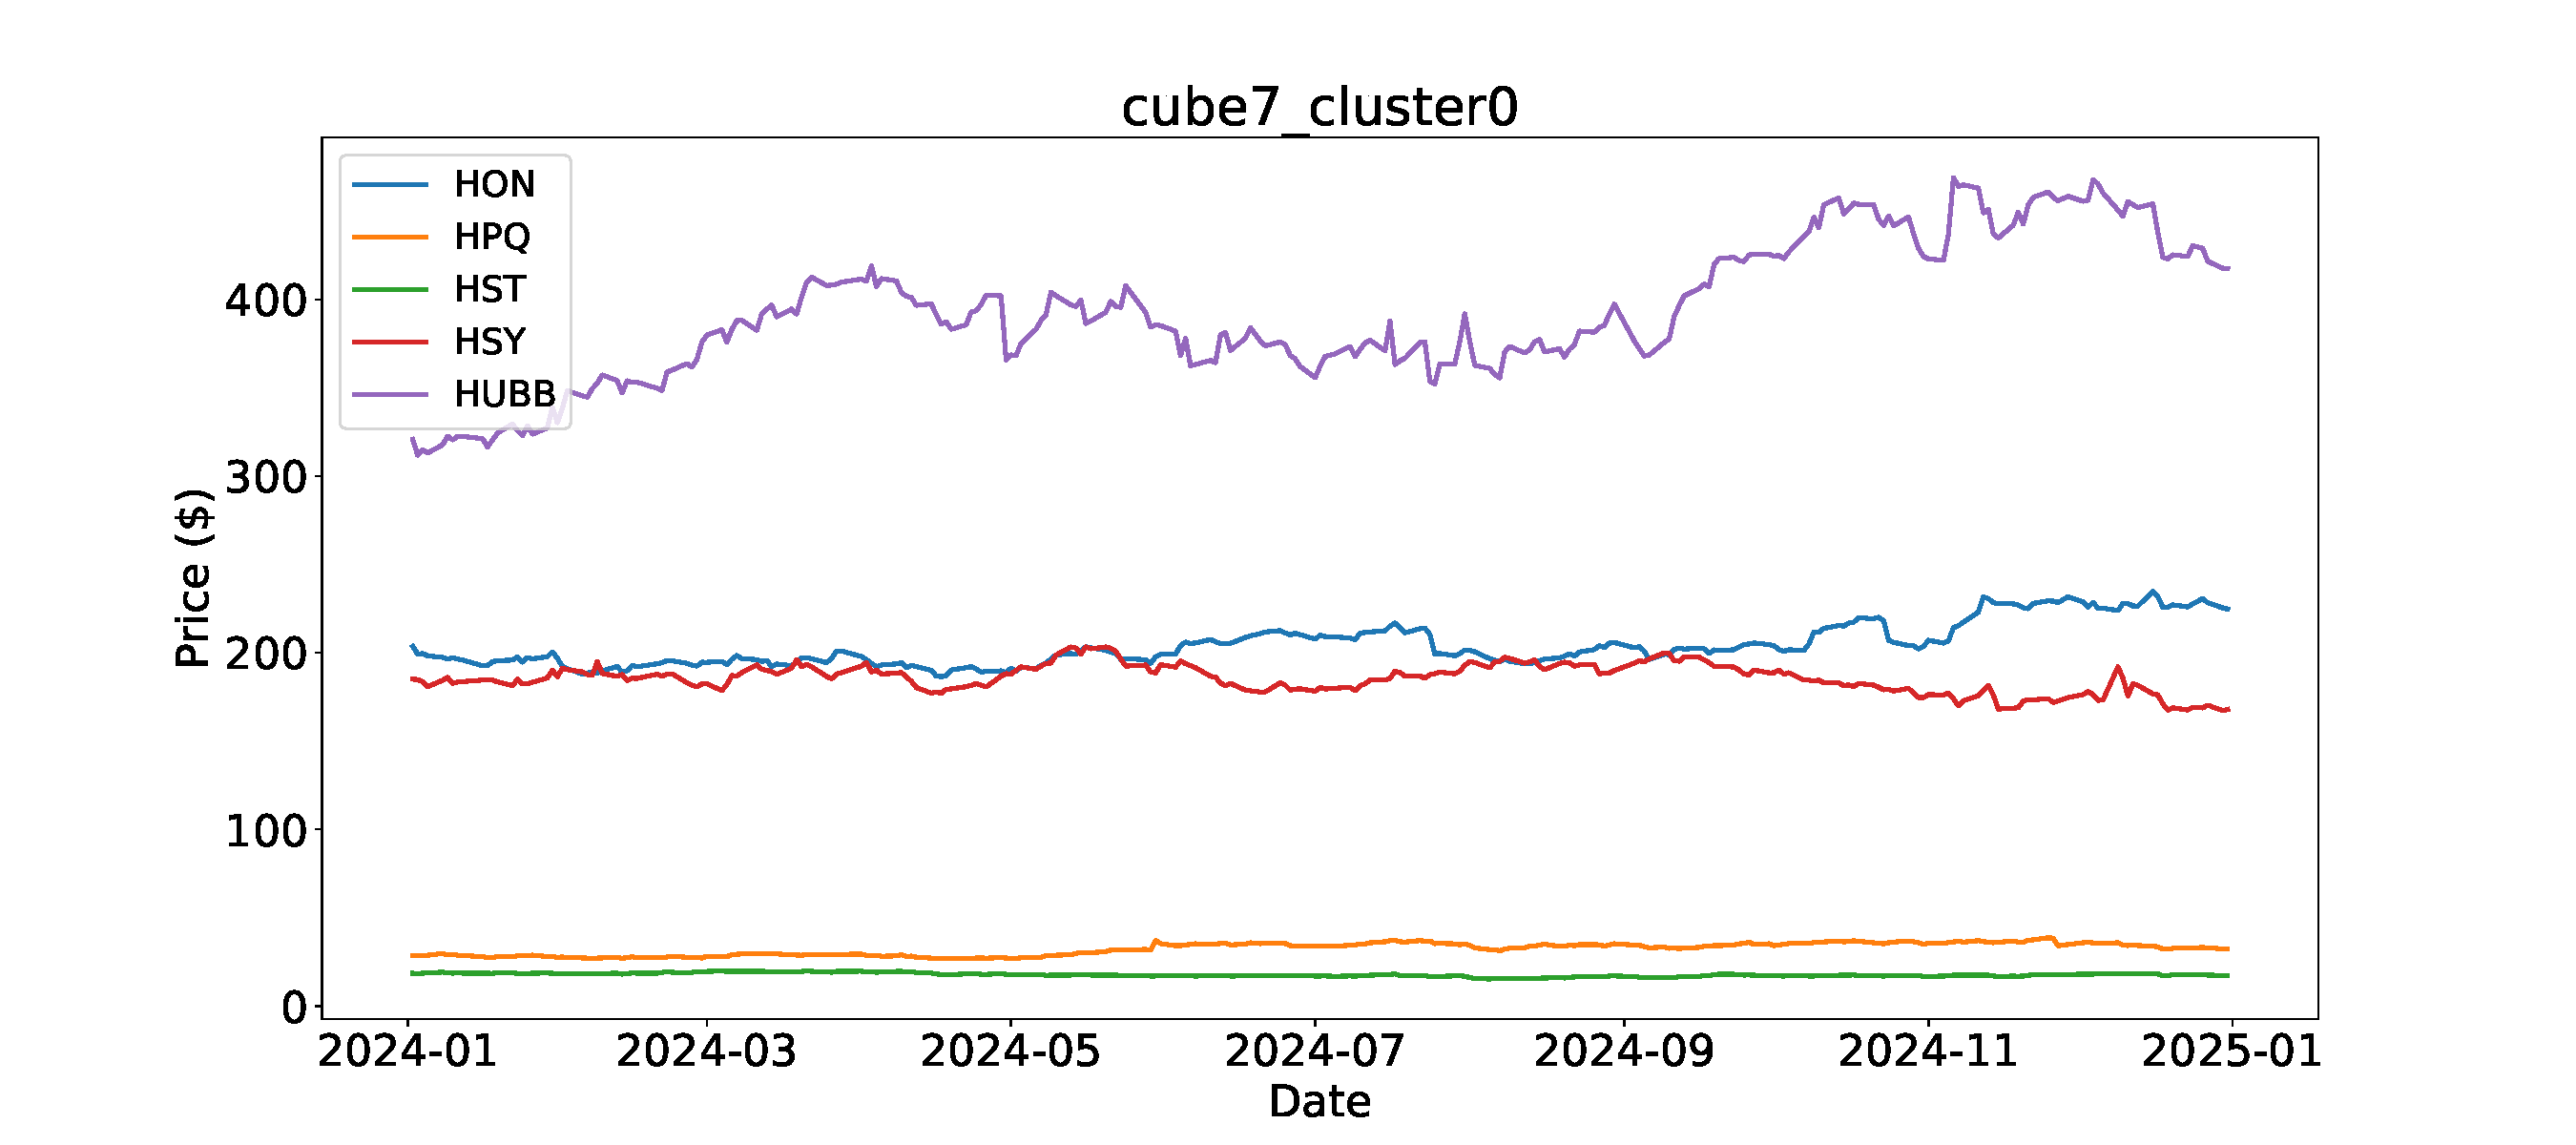
\includegraphics[width=14cm, height=10cm]{mapper_volatility_high_projection=UMAP_n_cubes=10_perc_overlap=0.1_clusterer=DBSCAN_scaler=MinMaxScaler.pdf}
  \caption{Cluster of tickers with the highest maximal volatility.}
  \label{fig:mapper_volatility_high}
\end{figure}

On first glance, the closing prices of the bottom four tickers do not seem highly volatile due to the wide price range we are plotting them against. Zooming on one of them, for example HPQ -- the ticker of the HP company known for printers -- reveals a more interesting structure in \ref{fig:mapper_volatility_hpq}.

\begin{figure}[h!]
  \centering
  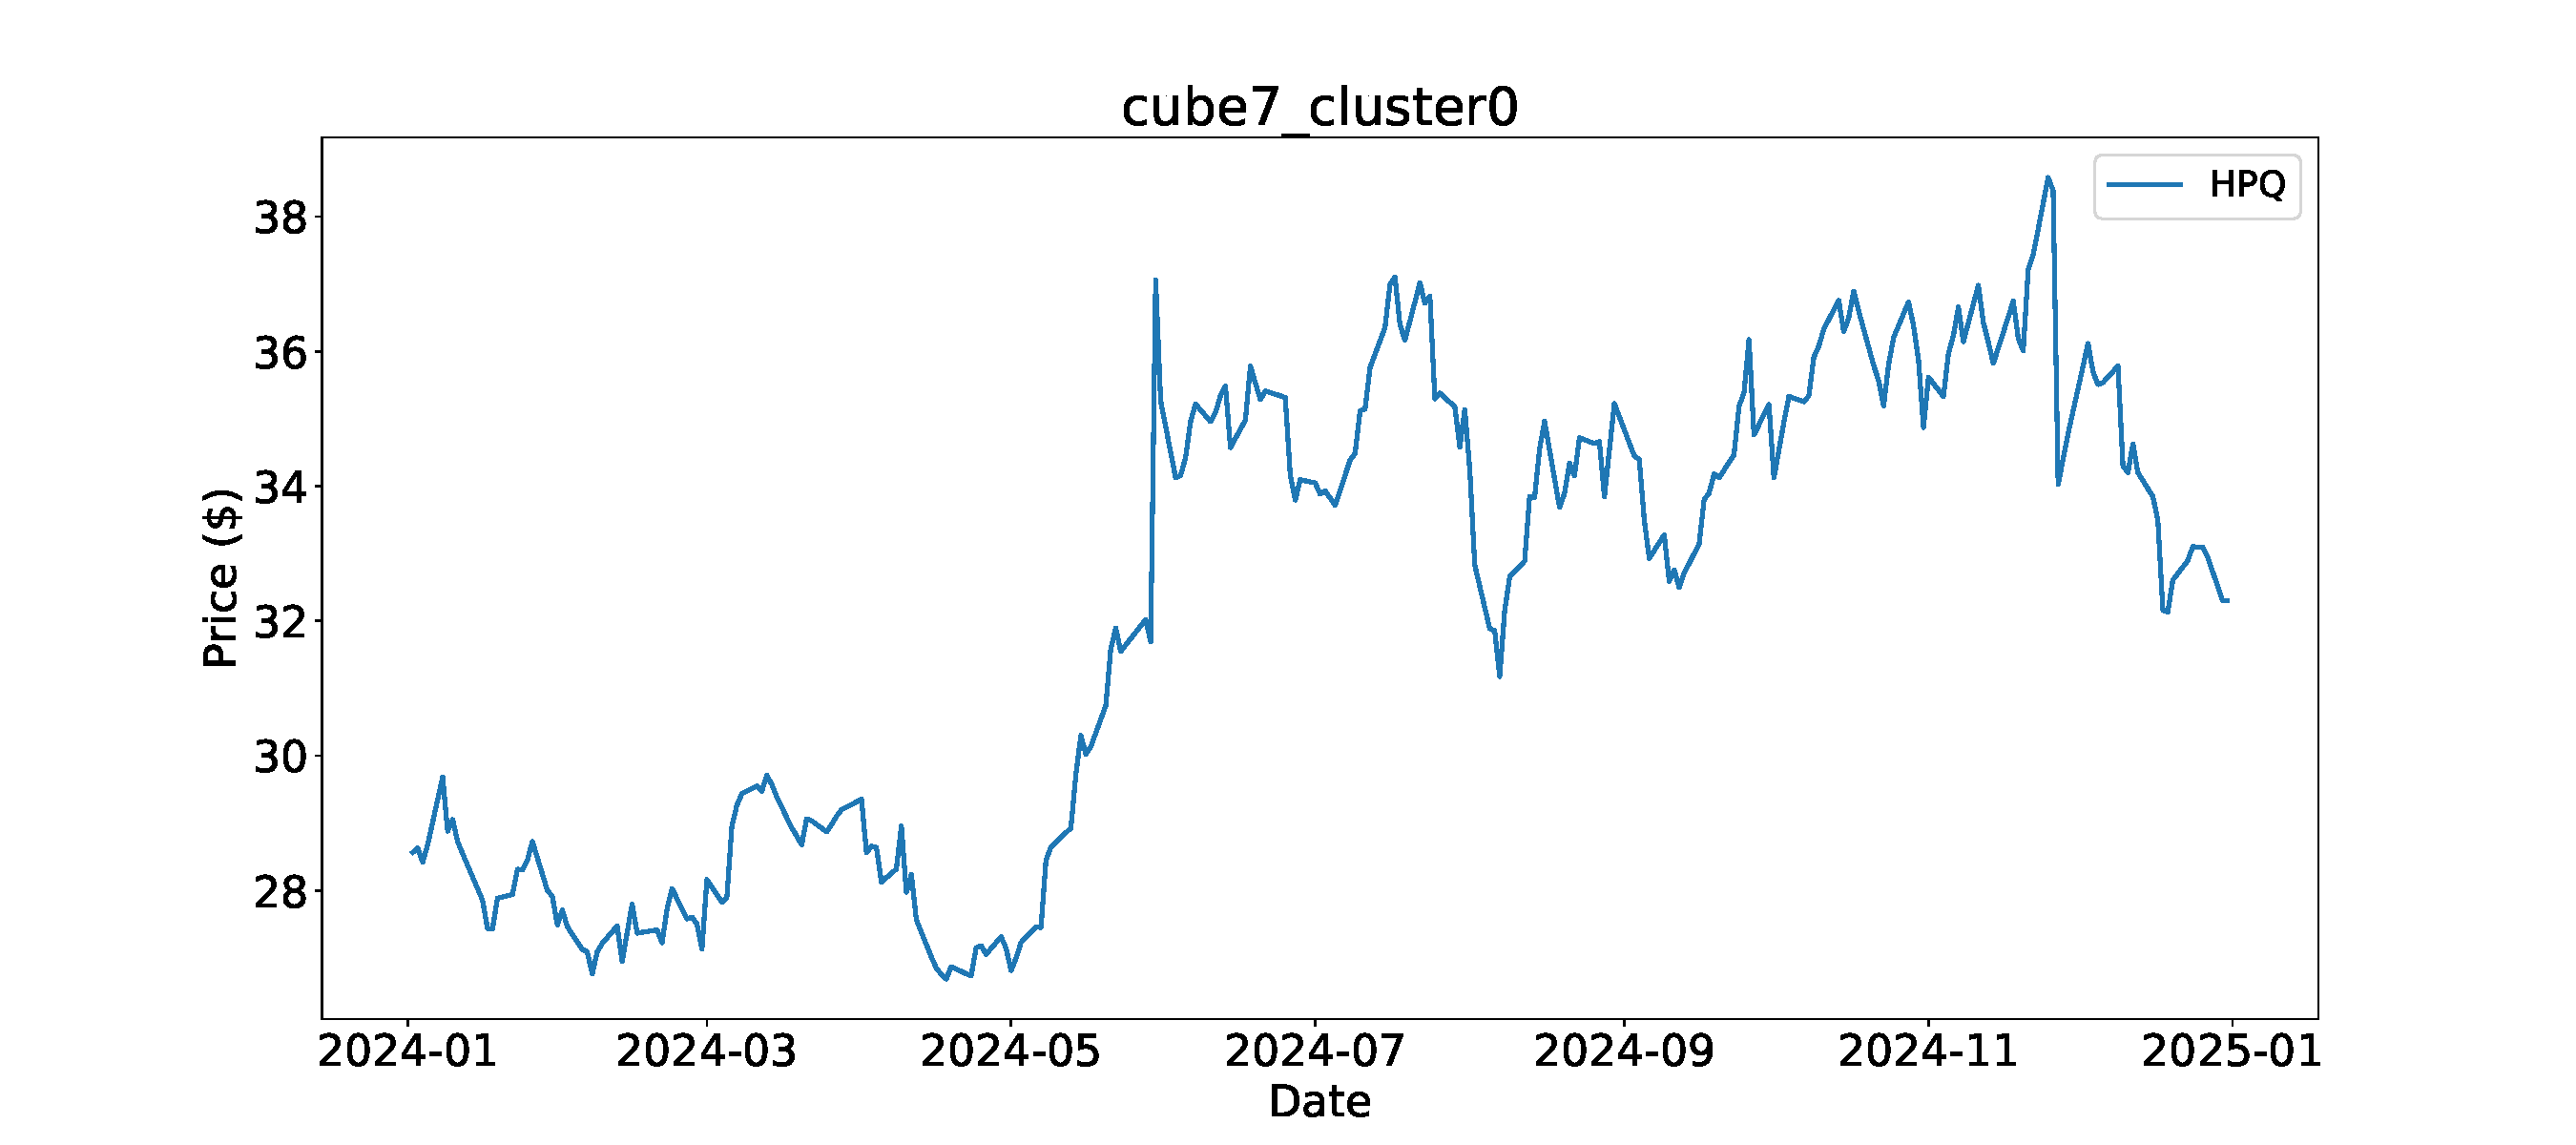
\includegraphics[width=14cm, height=10cm]{mapper_volatility_HPQ_projection=UMAP_n_cubes=10_perc_overlap=0.1_clusterer=DBSCAN_scaler=MinMaxScaler.pdf}
  \caption{Stock prices of the company HP during 2024-2025.}
  \label{fig:mapper_volatility_hpq}
\end{figure}

One could then continue with a more refined and detailed analysis of the clusters we obtained, looking into the differences and common points between them. Different coloring functions and rules could also be used, alongside other projection and clustering algorithms. All this is to show that Mapper is a powerful tool in the hands of someone with industry and theoretical knowledge of the data they have to work with, allowing them to carefully choose which algorithms, metrics and coloring functions they believe to be of importance.

\subsection{Digits dataset, revisited}
